% \chapter{Methods and data}

\chapter{Modelling renewable energy technologies}
\label{methods_physical}

\vspace{-15pt} % -15pts for two-line heading, -45pts for single-line heading
\begin{tcolorbox}[enhanced,width=\textwidth,size=fbox,
        sharp corners,colframe=black!5!white,drop fuzzy shadow southeast,
        boxrule=3mm, parbox=false] 
        
This chapter borrows from the articles \citep{walch_big_2020,walch_quantifying_2021}:

\qquad \bibentry{walch_big_2020}

\qquad \bibentry{walch_quantifying_2021}
\end{tcolorbox}

Spatio-temporal modelling of renewable energy potentials integrates physical models of the renewable resources and technologies with geospatial operations using Geographic Information Systems (GIS).
The present chapter introduces state-of-the-art modelling approaches for two types of renewables addressed in this thesis, namely rooftop solar energy (Section \ref{method_solar}) and shallow geothermal energy (Section \ref{geo_method}). 
\nomenclature[A]{GIS}{Geographic Information Systems}
Relevant physical, geographical and technical constraints for both energy resources are outlined and popular modelling approaches are summarized, such as to justify the methods used in the large-scale estimation of rooftop solar potential (Chapter \ref{solar}) and shallow geothermal potential (Chapter \ref{geothermal}).

\section{Rooftop solar energy}
\label{method_solar}
\label{method_solar_hierarchy}
% and solar thermal 

Rooftop solar energy is defined here as the electrical or thermal energy harvested from installations on building rooftops, using solar photovoltaic (PV) panels or solar thermal collectors (STC), respectively. 
While we focus on the estimation of solar photovoltaic (PV) potential, which is currently the most frequently deployed solar technology on rooftops \cite{kaufmann_schweizerische_2017}, most parts of the methodology (except the techological model of the solar PV panels) are transferable to STC. 
\nomenclature[A]{STC}{Solar thermal collector}
\nomenclature[A]{RPV}{Rooftop photovoltaics}
This section reviews state-of-the-art approaches to model the hourly energy yield of rooftop-mounted solar PV systems in the context of large-scale potential studies, and justifies the choice of the empirical models (Section~\ref{phys_models}), geospatial techniques (Section~\ref{GIS_methods}) and the modelling approach for PV panels on flat roofs (Section~\ref{app_flat}) used in the large-scale rooftop PV potential estimation presented in Chapter~\ref{solar}. We hereby do not claim to provide a complete review of existing modelling approaches, but rather give an overview of the relevant modelling steps and outline popular computational methods for each step.

\begin{figure}[tb]
	\centering
	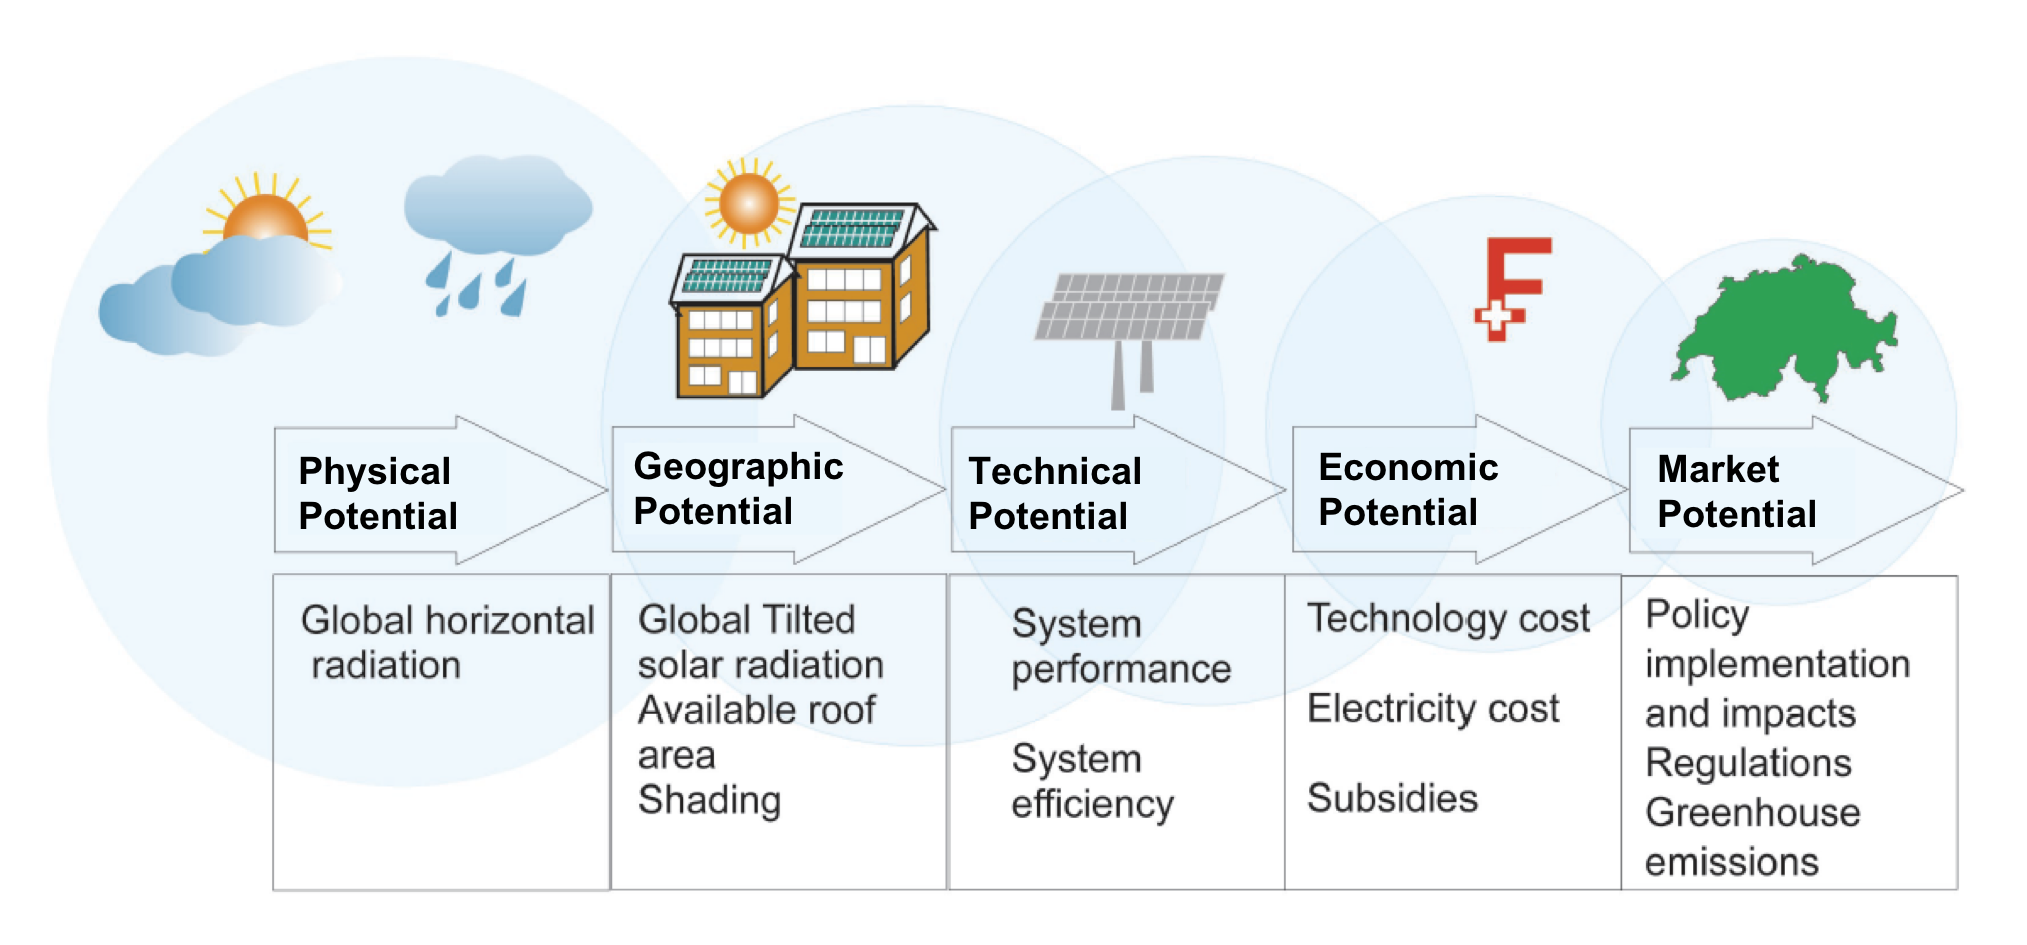
\includegraphics[width=\linewidth]{images/Figs/hierarchy.png}  
	\caption{Hierarchical approach for estimating rooftop PV potential. Source: \citet{assouline_estimation_2017}}
	\label{fig:solar_hierarchy}
\end{figure}

% SOURCE: CISBAT comparison paper
To compute the technical rooftop PV potential,  a hierarchical approach, shown in Fig.~\ref{fig:solar_hierarchy}, has been widely accepted in the literature \cite{assouline_quantifying_2017,ramirez_camargo_spatio-temporal_2015,izquierdo_method_2008,wiginton_quantifying_2010}. It includes (i) \textit{physical potential}, that is, the amount of solar energy reaching the earth’s surface, (ii) \textit{geographic potential}, that is, the amount of solar radiation received by the tilted PV panels, which is affected by the geometry of the panel (slope and aspect), the shading from surrounding buildings and trees and the suitable area for the panel installation, and (iii) \textit{technical potential}, that is, the maximum electricity output considering the technical characteristics of the PV technology (e.g. efficiency and system performance).

After obtaining the maximum feasible electricity output, one may consider additional environmental, economic or social considerations to refine the estimated size of the system. A fourth step may thus be an \textit{economic potential} focused on sizing the systems under given constraints. Economic considerations such as technology cost are not taken into account in most large-scale studies. Instead, these are typically assessed in separate studies that use the technical PV potential as input, in smaller-scale case studies as well as in hybrid potential assessments. An analysis of \textit{market potential} is beyond the scope of this work. 

\textbf{Physical potential.} The incoming solar radiation (also referred to as irradiance, in W/m$^2$), consists of three compotents: (i) a direct or beam component ($G_B$), which describes the direct incoming solar radiation on a horizontal plane, (ii) a diffuse component ($G_D$), which is diffracted for example through the atmosphere and through cloud coverage, and (iii) a surface reflected component $G_R$, which is driven by the ground surface reflectance, also known as albedo ($\rho$), but which can be omitted for horizontal planes \cite{assouline_estimation_2017}. Omitting $G_R$, the global horizontal solar radiation $G_h$ is given by \cite{assouline_estimation_2017}:

\begin{equation}
\label{eq:Gh_method}
G_{h} = G_{B} + G_{D}
\end{equation}

While most large-scale studies of RPV potential use satellite data or station measurements to obtain $G_h, G_B, G_D$ (e.g. \cite{bodis_high-resolution_2019,buffat_scalable_2018,ramirez_camargo_spatio-temporal_2015,calcabrini_simplified_2019}), empirical models exist to derive these from related variables such as the sunshine duration and the extra-terrestrial solar radiation \cite{assouline_estimation_2017}. 
In other cases, (geo)-statistical methods have been developed to estimate solar radiation. 
These include averaging the nearest neighbours \cite{klauser_solarpotentialanalyse_2016}, geostatistical methods such as kriging \cite{alsamamra_comparative_2009,rehman_spatial_2000} as well as machine learning approaches such as Support Vector Machines \cite{assouline_quantifying_2017}, Random Forests \cite{assouline_large-scale_2018} and neural networks \cite{hocaoglu_hourly_2008,notton_neural_2013,sahin_application_2013}. As averaging tends to oversimplify the modelling, and kriging is computationally intensive and requires modelling of anisotropic spatial correlations and stationarity of the process, the data-driven machine learning algorithms have recently gained much attention due to their performance and speed \cite{kanevski_machine_2009}. 
Most models do not estimate the uncertainty related to modelling horizontal irradiance, which is an important aspect if the results are processed further.
A further review of different modelling techniques for horizontal solar radiation is provided in \cite{zhang_review_2018}.

\textbf{Geographic potential.} The solar power received by RPV panels is driven by two factors: (i) the incoming solar radiation on the tilted panels, and (ii) the available area for installing PV, sometimes also quantified as the number of panels that can be installed on a rooftop. As the global horizontal radiation, the tilted radiation ($G_t$) is composed of a direct ($G_{Bt}$), a diffuse ($G_{Dt}$) and a reflected ($G_{Rt}$) component, such that \cite{assouline_estimation_2017}:

\begin{equation}
\label{eq:POA}
G_{t} = G_{Bt} + G_{Dt} + G_{Rt}
\end{equation}

The three components in Eq.~\ref{eq:POA} describe the plane-of-array (POA) radiation, obtained from empirical models (Section~\ref{phys_models}), which represents the radiation received by a fully unshaded PV panel in an open space. 
In urban environments, however, direct shading and a reduced sky visibility from surrounding buildings or other built-up objects, referred to as the sky view factor (SVF), can significantly impact the electricity yield of a PV panel. 
Hence, many studies of rooftop PV potential use geospatial techniques based on 2D or 3D models of the urban environment, detailed in Section~\ref{GIS_methods}, to quantify shading effects and the SVF (e.g.~\cite{desthieux_solar_2018,calcabrini_simplified_2019,wegertseder_combining_2016,jakubiec_method_2013}).
As these are included across the literature in the form of different factors, partially due to different spatial and temporal resolutions of RPV studies, we do not provide a generalised formulation to include these factors in Eq.~\ref{eq:POA}. However, in Chapter~\ref{solar_comparison} we will attempt to formulate such a generalisation for studies carried out in Switzerland.

The available area for installing PV or STC ($A_{PV}$) is potentially the factor that varies most between different studies of RPV potential, as it is strongly dependent on the scale of the study and on the available rooftop data. 
Rooftop available area is either quantified as constant factors (e.g. \cite{iea_potential_2002,wegertseder_combining_2016,portmann_sonnendach.ch:_2016}) or derived from building data (\cite{ramirez_camargo_spatio-temporal_2015,assouline_quantifying_2017,hong_development_2017}) and aerial imagery \cite{mainzer_assessment_2017} using geospatial techniques or image processing. 
As the required geospatial input data may not be available across entire study areas and the computational time for these methods may be prohibitively high, sampling techniques \cite{izquierdo_method_2008}, the use of building prototypes \cite{wegertseder_combining_2016} and extrapolation techniques using ML \cite{assouline_quantifying_2017,assouline_large-scale_2018} based on geospatial methods are frequently used in large-scale studies. 
A review of statistical and geospatial techniques for quantifying the available roof area is provided in Section~\ref{GIS_methods}, while constant factors used in the literature are compared in \cite{assouline_estimation_2017,wiginton_quantifying_2010,singh_estimation_2015}.

\textbf{Technical potential.} The conversion of global radiation to PV potentials is driven by three factors: the efficiency of the PV panel ($\eta_{PV}$), the inverter efficiency ($\eta_\mathit{inv}$) and other losses ($\eta_\mathit{losses}$), which are multiplied with the tilted radiation ($G_t$) and the available area for PV installation ($A_{PV}$):

\begin{equation}
    P_{PV} = G_t \times A_{PV} \times \eta_{PV} \times \eta_\mathit{inv} \times \eta_\mathit{losses}
\end{equation}

While several studies use constant values for panel and inverter efficiencies \cite{assouline_quantifying_2017,wegertseder_combining_2016,romero_rodriguez_assessment_2017,ordonez_analysis_2010,hong_development_2017}, many high-resolution PV potential studies use analytical or empirical models to quantify the efficiencies as a function of radiation, temperature, wind speed and technical characteristics of PV systems. The level of detail of these models ranges from the analytical modelling of invidual cells and their arrangement in a PV panel \cite{buffat_scalable_2018} to entirely coefficient-based empirical models \cite{mainzer_assessment_2017} (see Section~\ref{phys_models}). Other losses, however, are accounted for as constant loss factors in most studies. These may account for panel soiling, degradation, network and wiring losses, partial shading of panels and other factors.

An overview of the parameters used to estimate the physical, geographic and technical PV potential and a summary of methods to compute these is provided in Table~\ref{tab:solar_methods_compare}.

\begin{table}[htbp]
\centering
\footnotesize
\caption{Parameters for estimating the physical, geographic and technical potential and a (non-exhaustive) review of methods to compute these parameters.}
\label{tab:solar_methods_compare}
\resizebox{\textwidth}{!}{%
\begin{tabular}{llllll}
\hline
\textbf{Type} & \textbf{Parameters} & \textbf{Unit} & \textbf{Description} & \textbf{Methods (selected)} & \textbf{References} \\ \hline
\multirow{4}{*}{\begin{tabular}[c]{@{}l@{}}\textit{Physical}\\ \textit{potential}\end{tabular}} & \multirow{4}{*}{$G_h, G_B, G_D$} & \multirow{4}{*}{W/m$^2$} & \multirow{4}{*}{\begin{tabular}[c]{@{}l@{}}Global, direct, diffuse\\ horizontal solar radiation\end{tabular}} & Satellite / measured data & \cite{bodis_high-resolution_2019,buffat_scalable_2018,ramirez_camargo_spatio-temporal_2015,calcabrini_simplified_2019} \\
 &  &  &  & Empirical models & \cite{assouline_estimation_2017} \\
 &  &  &  & Kriging &  \cite{alsamamra_comparative_2009,rehman_spatial_2000}  \\
 &  &  &  & Machine Learning & \cite{assouline_quantifying_2017,assouline_large-scale_2018,hocaoglu_hourly_2008,notton_neural_2013,sahin_application_2013} \\ \hline
\multirow{11}{*}{\begin{tabular}[c]{@{}l@{}}\textit{Geographic}\\ \textit{potential}\end{tabular}} & $G_t$ & \multirow{4}{*}{W/m$^2$} & Tilted (POA) radiation & $G_t = G_{Bt} + G_{Dt} + G_{Rt}$ &  \\
 & $G_{Bt}, G_{Rt}$ &  & Direct, reflected component & Geometric projection & \cite{gulin_estimation_2013} \\
 & \multirow{2}{*}{$G_{Dt}$} &  & \multirow{2}{*}{Diffuse component} & Perez model & \cite{perez_modeling_1990, buffat_scalable_2018,jakubiec_method_2013,mainzer_assessment_2017,wegertseder_combining_2016} \\
 &  &  &  & Other (Hay, Liu-Jordan, Klein) & \cite{desthieux_solar_2018,izquierdo_method_2008,singh_estimation_2015, assouline_estimation_2017}  \\ \cline{2-6} 
 & \multirow{3}{*}{\begin{tabular}[c]{@{}l@{}}SVF / \\ Shading\end{tabular}} & \multirow{3}{*}{-} & \multirow{3}{*}{\begin{tabular}[c]{@{}l@{}}Sky view factor /\\ Shaded roof area\end{tabular}} & Fisheye images &  \cite{calcabrini_simplified_2019}\\
 &  &  &  & Digital surface model/LiDaR & \cite{jakubiec_method_2013,desthieux_solar_2018,hong_development_2017,strzalka_large_2012} \\
 &  &  &  & Roof fraction (constant) & \cite{mainzer_assessment_2017,wiginton_quantifying_2010, izquierdo_method_2008} \\ \cline{2-6} 
 & \multirow{4}{*}{APV} & \multirow{4}{*}{m$^2$} & \multirow{4}{*}{Available roof area} & Entire roof area & \cite{ramirez_camargo_spatio-temporal_2015,buffat_scalable_2018,hong_development_2017} \\
 &  &  &  & Roof fraction (constant) & \cite{iea_potential_2002,wegertseder_combining_2016,portmann_sonnendach.ch:_2016,wiginton_quantifying_2010}  \\
 &  &  &  & Derived from geospatial data & \cite{assouline_large-scale_2018,ordonez_analysis_2010, mainzer_assessment_2017} \\
 &  &  &  & Extrapolation to the large-scale & \cite{izquierdo_method_2008, wegertseder_combining_2016,assouline_quantifying_2017} \\ \hline
\multirow{4}{*}{\begin{tabular}[c]{@{}l@{}}\textit{Technical}\\ \textit{potential}\end{tabular}} & \multirow{2}{*}{$\eta_{PV}, \eta_{\mathit{inv}}$} & \multirow{2}{*}{-} & \multirow{2}{*}{\begin{tabular}[c]{@{}l@{}}PV panel, inverter \\ efficiency\end{tabular}} & Empirical model & \cite{jakubiec_method_2013,ramirez_camargo_spatio-temporal_2015,lukac_buildings_2014,buffat_scalable_2018,mainzer_assessment_2017,calcabrini_simplified_2019} \\
 &  &  &  & Constant value &  \cite{wegertseder_combining_2016,romero_rodriguez_assessment_2017,ordonez_analysis_2010,assouline_quantifying_2017,hong_development_2017,bodis_high-resolution_2019} \\
 & $\eta_{\mathit{losses}}$ & - & \begin{tabular}[c]{@{}l@{}}System losses (Soiling, wiring,\\ degradation etc.)\end{tabular} & Constant value & \cite{klauser_solarpotentialanalyse_2016,buffat_scalable_2018,mainzer_assessment_2017,lorenz_regional_2011,bodis_high-resolution_2019} \\ \hline
\end{tabular}
}
\end{table}

\begin{comment}
The panel efficiency is dependent on the selected technology and lies typically between 15-20\%. The performance ratio considers several external factors affecting the system’s performance, such as operating temperature, panel obstruction or converter losses. It can thus be calculated using an analytical formula [9], in most large-scale studies it is however approximated as 80\% [3], [5], [6]. Given the global irradiance on tilted surfaces Gt, the useful rooftop area AR, the power factor PF and the panel efficiency $\eta_{PV}$, the total PV power output per rooftop $P_{PV}$ (in $W$) can hence be calculated as:
\end{comment}

\subsection{Empirical models}
\label{phys_models}

Empirical models are widely used in the modelling of the electricity yield of RPV systems, as they allow to estimate relevant physical variables with little computational effort and from widely available data. 
In particular, empirical models are used in the literature (i) to quantify the plane-of-array (POA) radiation, namely the tilted radiation components ($G_{Bt}, G_{Dt}, G_{Rt}$) incident to the inclined PV panels, and (ii) for modelling solar PV technology, more specifically the efficiency of the PV panel and the inverter, which converts the direct current (DC) PV output to "grid-level" alternating current (AC). 

%% SOURCE: Research plan
%To compute the potential energy output, firstly the amount of solar power reaching a tilted panel/collector surface must be computed. This quantity is defined as global solar irradiance and given in W/m2. It consists of 3 components: a direct or beam component, a diffuse component and a reflected component (see Figure 3a). They are calculated from measurements of global horizontal (GHI), direct normal (DNI) and diffuse horizontal irradiance (DHI). Direct normal irradiance is converted to the tilted beam component via a geographic projection shown in Figure 3b. Diffuse tilted irradiance is more complex to determine due to its diffracted nature. Several models exist with different assumptions and hence varying complexity. Gueymard [15] compared several of these models and compared their approximation errors under different operating conditions. While no model clearly outperforms the other models, his analysis shows the Klucher method [16] amongst the best in most scenarios. The reflected component is given by another geometric conversion based on the ground’s surface reflectance. The mathematical formulae for the conversions are demonstrated for example by Gulin et al. [17].

% Figure 3: a) three solar irradiance components reach a solar panel: direct (beam), diffuse and reflected irradiance; b) geometry for calculating the angle of incidence of direct beam irradiance on a tilted plane;  , : surface tilt & azimuth, z : apparent sun zenith,  : angle of incidence [17]

\subsubsection{Plane-of-array radiation}
\label{app:irrad}

\begin{figure}[bt]
\centering
\begin{subfigure}[t]{.43\textwidth}
  \centering
  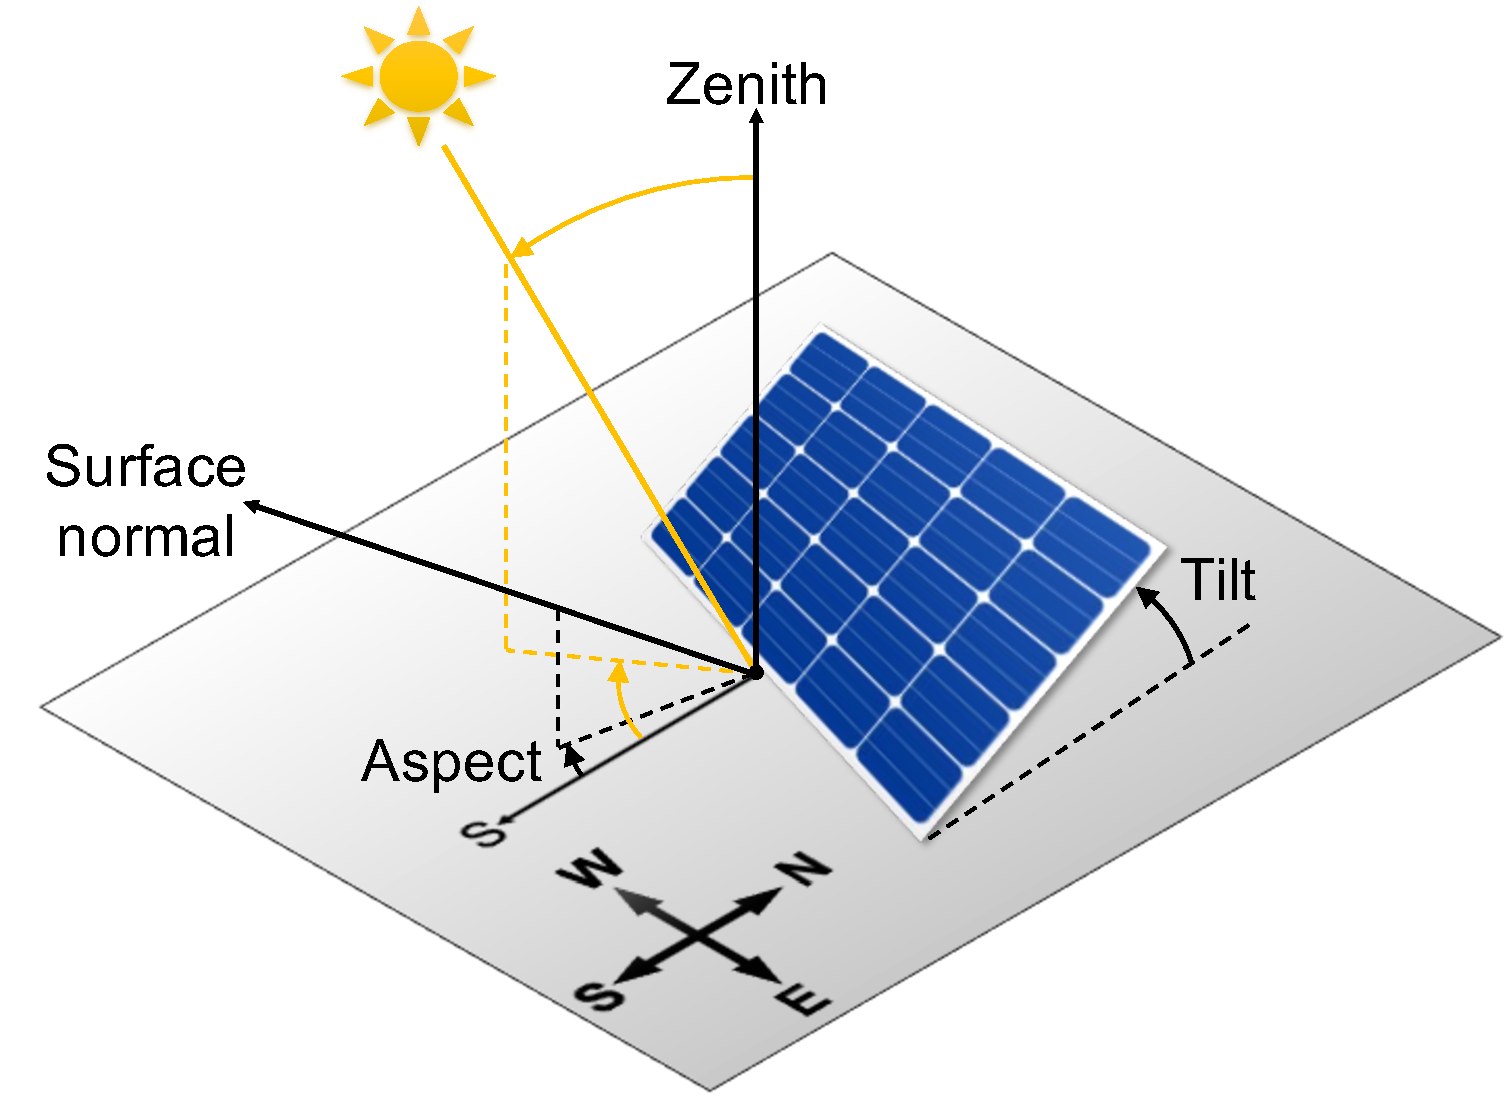
\includegraphics[width=\linewidth]{images/Figs/poa.pdf}  
    \subcaption{}
  \label{figa:solar_geom}
\end{subfigure}
\begin{subfigure}[t]{.53\textwidth}
  \centering
  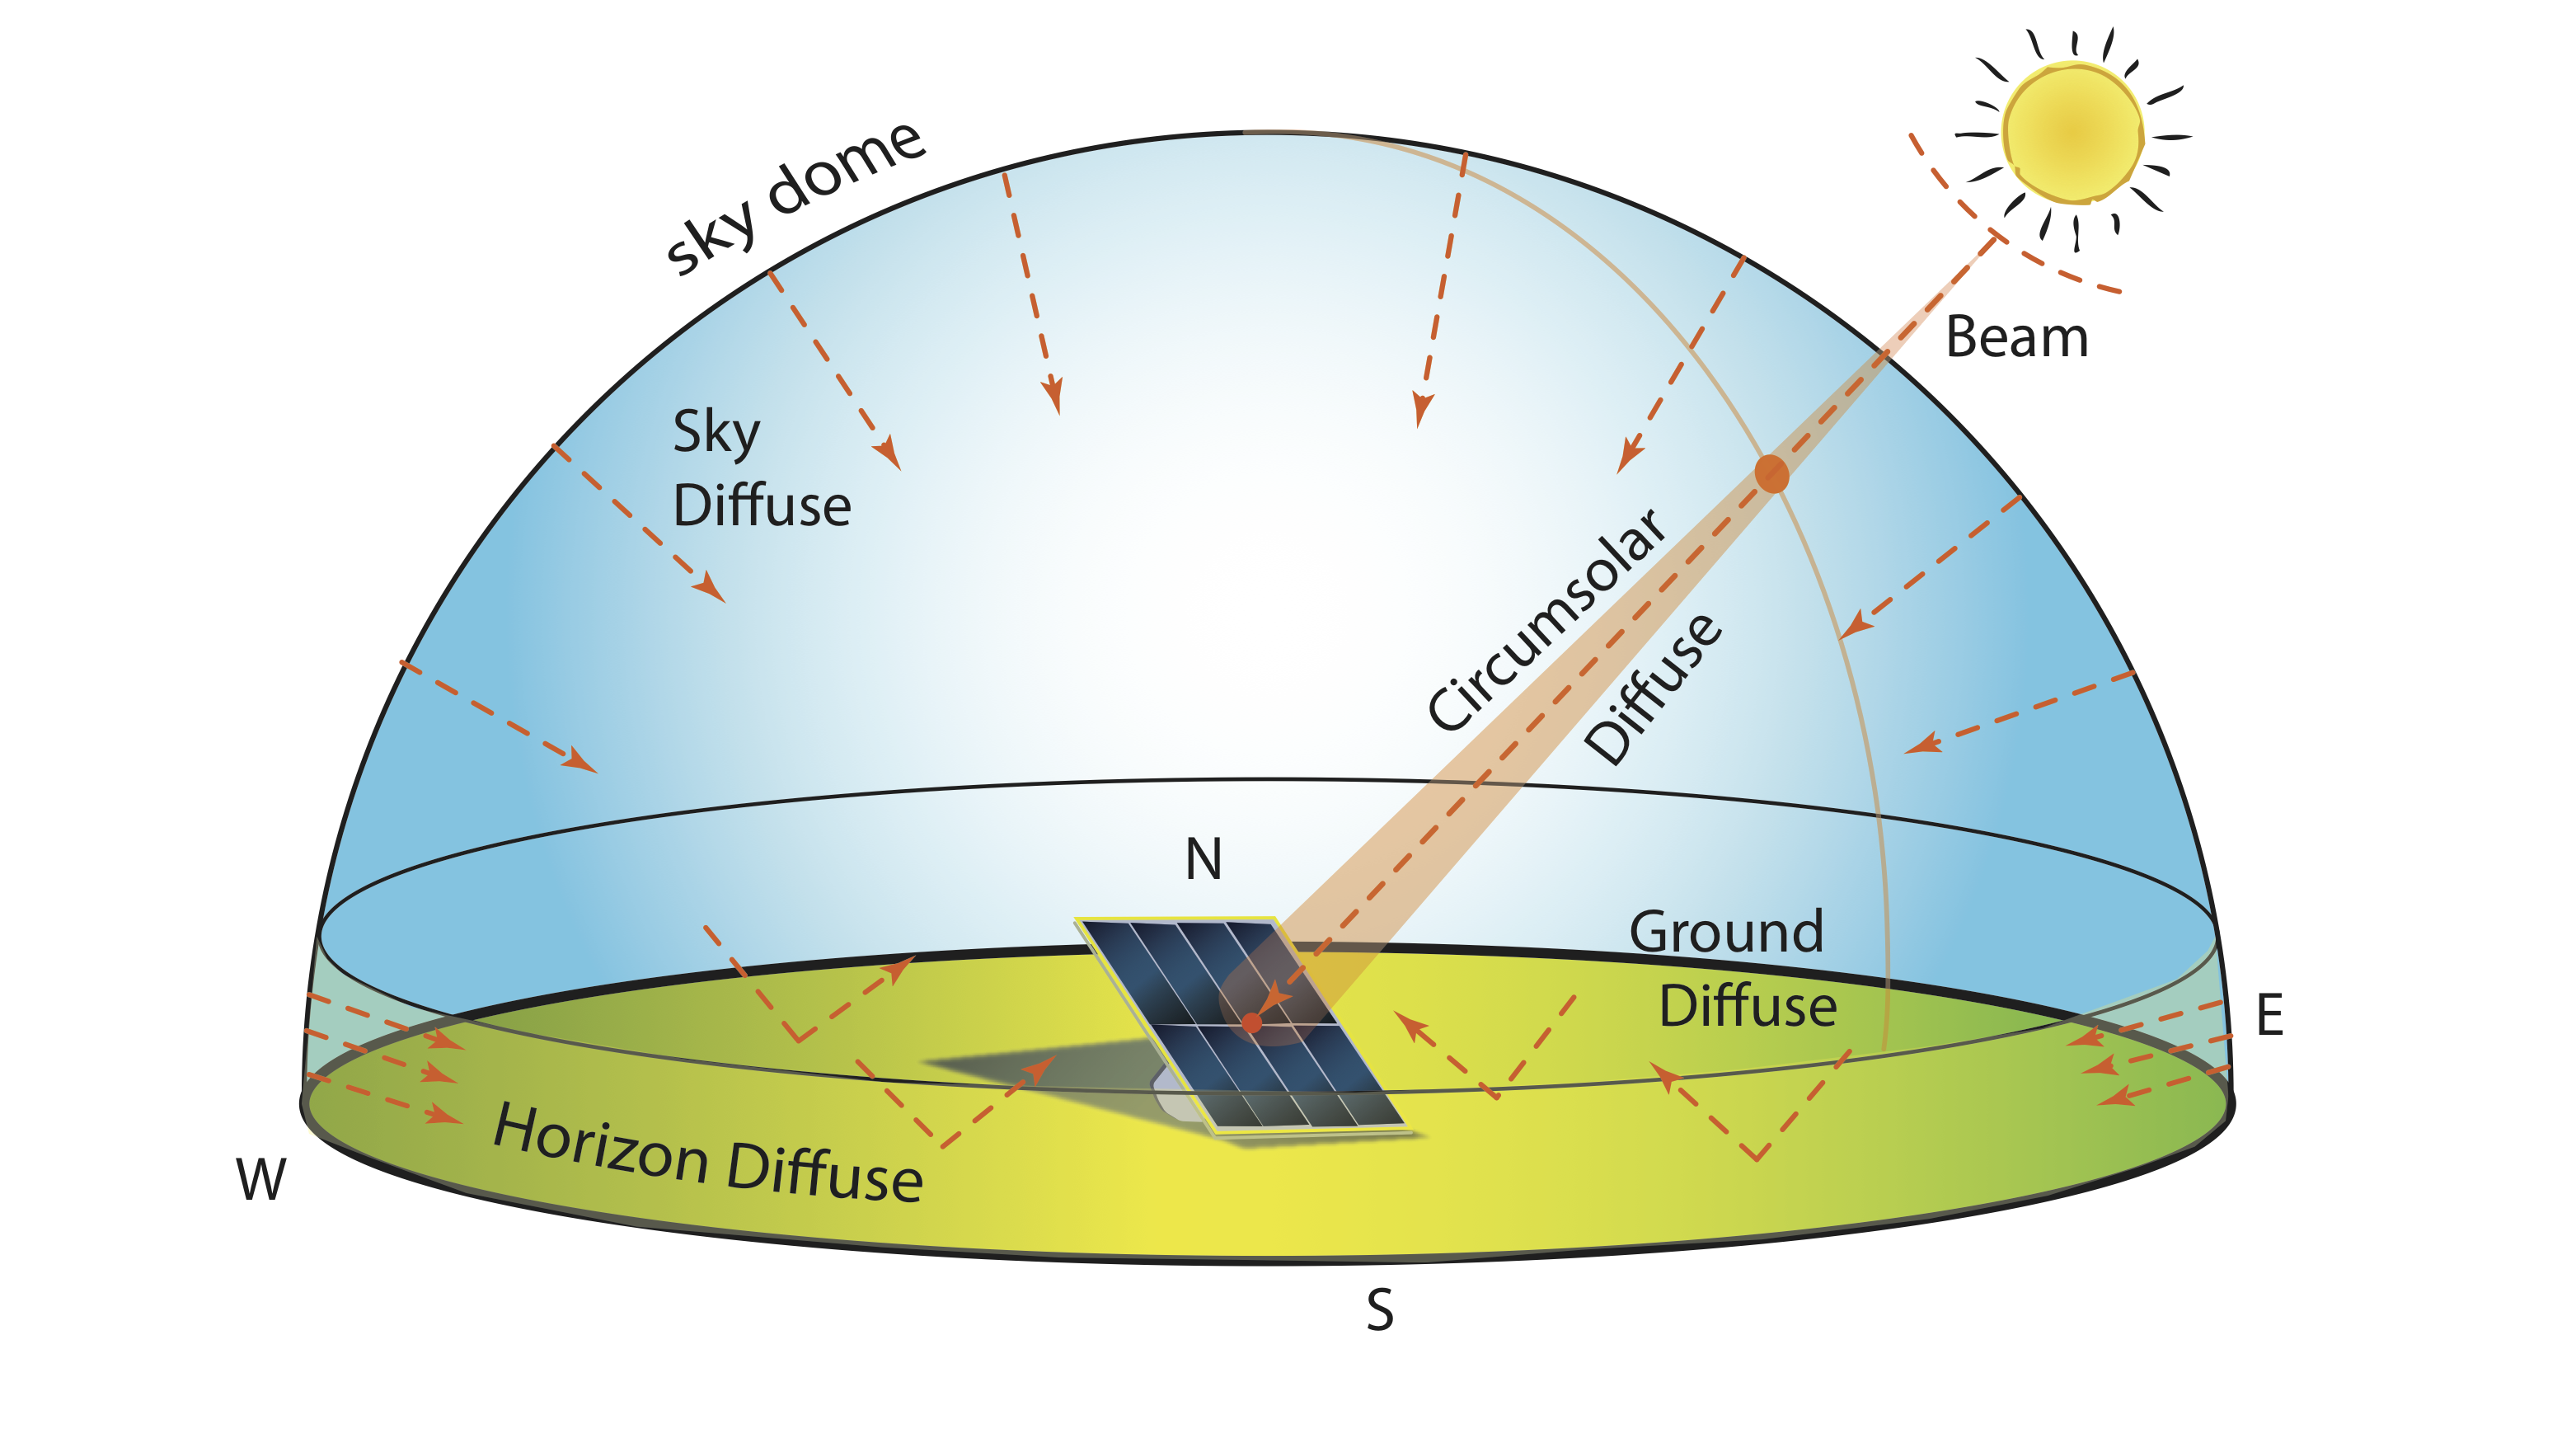
\includegraphics[width=\linewidth]{images/Figs/diffuse_components.png}  
    \subcaption{}
  \label{figb:solar_geom}
\end{subfigure}
\caption{Geometrical models for calculating (a) the angle of incidence of direct beam radiation on a tilted plane, and (b) the isotropic, circumsolar and horizon diffuse components (Source: \citet{brownson_44_nodate}).}
\label{fig:solar_geom}
\end{figure}

To compute the direct, diffuse and reflected tilted irradiance components $G_{Bt}$, $G_{Dt}$ and $G_{Rt}$, empirical and geometrical models are widely accepted in the literature. 
The direct component is obtained from a geometrical projection of the horizontal $G_B$ on the angle of incidence of the sun rays on the tilted panel ($\theta$) (see Fig.~\ref{figa:solar_geom}). Mathematicaly, this projection is defined as \cite{gulin_estimation_2013}:

\begin{equation}
\label{eq:direct}
    G_{Bt} = G_{B} * \max \left( 0, \frac{\cos(\theta)}{\cos(\theta_Z)} \right)
\end{equation}
where
\begin{equation}
\label{eq:dir_angle}
\cos(\theta) = \sin(\beta) \sin(\theta_Z) \cos(\gamma_S - \gamma) + \cos(\beta) \cos(\theta_Z) 
\end{equation}

The angles $\theta_Z$ and $\gamma_S$ describe the sun zenith and azimuth angles, respectively, while roof tilt and aspect are given by $\beta$ and $\gamma$.

Diffuse tilted irradiance is more complex to determine due to its diffracted nature. Several models exist with different assumptions and hence varying complexity. \citet{assouline_estimation_2017} review these different models and compares the temporal resolutions for which they are applicable.
Of the methods listed in \citet{assouline_estimation_2017} , the Perez model ~\cite{perez_modeling_1990} is the most frequently used model in the reviewed literature \cite{buffat_scalable_2018,jakubiec_method_2013,mainzer_assessment_2017,wegertseder_combining_2016}, and will also be used throughout this thesis.
The empirical formula for $G_{Dt}$ using the Perez model is given by~\cite{perez_modeling_1990}:

\begin{equation}
\label{eq:diffuse}
G_{Dt} = G_D * \left[ (1 - F_1) \left( \frac{1 + \cos \beta}{2} \right) 
       + F_1 \frac{ a }{ b }
       + F_2 \sin \beta \right]
\end{equation}

where $F_1$ and $F_2$ are empirically fitted functions for the circumsolar and horizon brightness, and $a$, $b$ are geometric angles. The derivation of these factors is described in \cite{loutzenhiser_empirical_2007}. The three addends in Eq.~\ref{eq:diffuse} represent an isotropic component, a circumsolar component originating from the sun disk (modelled as a point source) and a horizon component respectively, as shown in Fig.~\ref{figb:solar_geom}.

The reflected radiation ($G_{Rt}$) is again obtained from a widely used geometric projection based on the surface albedo $\rho$, which is defined as \cite{duffie_solar_2013}:

\begin{equation}
\label{eq:reflected}
G_{Rt} = G_h * \rho \left( \frac{1-\cos \beta}{2} \right)
\end{equation}

To ease the notation, Equations~\ref{eq:direct}-\ref{eq:reflected} can be referred to as:

\begin{equation}
\label{eq:tilted_irrad_simplified}
G_{Bt} = F_B G_B, \quad G_{Dt} = F_D G_D, \quad G_{Rt} = F_R G_h
\end{equation}



\subsubsection{PV module and inverter efficiency}
\label{app:efficiency}

In contrast to the modelling of the POA radiation, various empirical models exist to compute the electricity yield of PV systems. 
To compute the panel efficency ($\eta_{PV}$), the most detailed models simulate the maximum power point of the PV panel using single-diode current voltage equations \cite{strzalka_large_2012,buffat_scalable_2018}.
Most studies use a more generalised approach, which models $\eta_{PV}$ as a function of $G_t$, the PV cell temperature (derived from the ambient temperature) and the nominal performance rating of the PV panel \cite{jakubiec_method_2013,calcabrini_simplified_2019,singh_estimation_2015,ramirez_camargo_spatio-temporal_2015,mainzer_assessment_2017}. \citet{jakubiec_method_2013} compare PV efficiency models for widely used tools for two test buildings.

A general formulation of the DC power output of a PV panel ($P_{dc}$) is formulated in the \textit{PVWatts} model developed by the National Renewable Energy Laboratory (NREL) \cite{dobos_pvwatts_2014}, which is used in similar formulations for example in \cite{jakubiec_method_2013,ramirez_camargo_spatio-temporal_2015,singh_estimation_2015,calcabrini_simplified_2019}. 
In this work, we follow these studies, modelling the DC power output of a PV panel as:

\begin{equation}
\label{eq:Pdc}
    P_{dc} = \frac{G_{t}}{1000} P_{dc0} (1 + \gamma_\mathit{pdc}(T_\mathit{cell}-T_\mathit{ref}))
\end{equation}

where $G_t$ is the tilted radiation, $P_{dc0}$ is the DC rating of the panel,  $\gamma_\mathit{pdc}$ is its temperature coefficient, $T_\mathit{cell}$ is the cell temperature and $T_\mathit{ref}$ is the reference temperature.
%
We use average panel specifications of mid-range 60-cell mono-crystalline PV modules, the most frequently used technology in Switzerland \cite{buffat_scalable_2018}, from three market-leading manufacturers (JA Solar, Jinko Solar, Trinasolar). The values are reported in Table~\ref{tab:efficiency}.
%
From the DC power output and the area of a PV panel ($A_\mathit{panel}$), the module efficiency $\eta_{PV}$ is computed as:

\begin{equation}
\label{eq:eff}
    \eta_{PV} = \frac{P_{dc}}{G_{t} * A_\mathit{panel} }
\end{equation}

\begin{table}[tb]
\centering
\footnotesize
\caption{Parameters used in the PV module and inverter efficiency models \cite{dobos_pvwatts_2014, faiman_assessing_2008}.}
\label{tab:efficiency}

    \begin{tabular}{lll}
    \hline
    \textbf{Parameter} & \textbf{Value}     & \textbf{Description}          \\ \hline
    $P_{dc0}$          & 285 Wp           & Nameplate DC rating           \\
    $\gamma_{pdc}$     & $-0.39$ \%/°C& Temperature coefficient       \\
    $T_{ref}$          & 25 °C       & Cell reference temperature    \\
    $\alpha$           & 0.9                & Absorption coefficient        \\
    $\eta_m$           & 0.17               & Nominal module efficiency     \\
    $U$                & 15 W/m$^2K$        & Heat transfer component       \\
    $A_\mathit{panel}$        & 1.6 m$^2$          & PV panel area                 \\
    $\eta_\mathit{nom}$       & 0.96               & Nominal inverter efficiency   \\
    $\eta_\mathit{ref}$       & 0.9637             & Reference inverter efficiency \\ \hline
    \end{tabular}
\end{table}

With the exception of \cite{calcabrini_simplified_2019}, $T_\mathit{cell}$ is computed in the literature as a linear combination of the ambient temperature $T_\mathit{amb}$ and $G_t$, whereby $G_t$ is multiplied with a constant coefficient based on nominal operating conditions and corrected for the roof absorptivity and radiative heat losses \cite{jakubiec_method_2013}.
%
In this work, we use the \textit{PVSyst} model~\cite{faiman_assessing_2008} to derive $T_\mathit{cell}$ from $G_t$ and $T_\mathit{amb}$:

\begin{equation}
    T_\mathit{cell} = T_\mathit{amb} + G_t \frac{\alpha (1 - \eta_m)}{U}
\end{equation}

where $\alpha$ denoted the absorption coefficient, $\eta_m$ denotes the module efficiency and $U$ is the heat transfer component, for which we use default values for rooftop-mounted PV systems as suggested by Sandia National Laboratories \cite{holmgren_pvlib_2018} (Table~\ref{tab:efficiency}).

In contrast to Eq.~\ref{eq:Pdc}, which is based on physical principles, the inverter effiency ($\eta_\mathit{inv}$) is modelled using a fully empirical formula with three free parameters. Out of the various sets of coefficients in the literature \cite{mainzer_assessment_2017,lukac_buildings_2014}, we use the empirical loss formula from \textit{PVWatts}, also used in \cite{buffat_scalable_2018}, for consistency with Eq.~\ref{eq:Pdc}. It is defined as \cite{dobos_pvwatts_2014}:

\begin{equation}
\label{eq:inv}
    \eta_{inv} = \frac{\eta_{nom}}{\eta_{ref}} \left( -0.0162 * \zeta - \frac{0.0059}{\zeta} + 0.9858 \right)
\end{equation}

where $\zeta = P_{dc}/P_{dc0}$, $\eta_{nom}$ is the nominal inverter efficiency and $\eta_{ref}$ is the reference efficiency (see Table \ref{tab:efficiency} for values used in this work). 
%
Multiplying  $\eta_{inv}$ with other system losses $\eta_\mathit{losses}$, including soiling, degradation, mismatch, wiring and connection losses, yields the performance factor (\textit{PF}) \cite{klauser_solarpotentialanalyse_2016}. 
These additional losses are estimated throughout this work as 14\% \cite{dobos_pvwatts_2014}. 
The implementation of the empirical models is based on the \texttt{pvlib} python package developed by Sandia National Laboratories \cite{holmgren_pvlib_2018}.

\subsection{Geospatial techniques}
\label{GIS_methods}

In the context of large-scale studies of solar PV potential, geospatial methods are used to accurately quantify shading effects, the sky view factor and the available area for PV installation. The primary inputs for these methods are 2D building or roof geometries in vector format, as well as 3D Light Detection and Ranging (LiDaR) point clouds or digital elevation models (DEM) in raster format. While LiDaR data has a higher spatial resolution and is hence used for building or neighbourhood-scale studies, DEMs are mostly used for studies at regional scale for reasons of computational efficiency. 

In the following, we summarize existing methods to compute shading, SVF and available area, with a focus on methods that are scalable to entire cities or regions.
Alternative approaches, including constant-value methods and extrapolation techniques, are reviewed in \cite{assouline_estimation_2017}.

\subsubsection{Shading effects and sky view factor}

\begin{figure}[tb!]
	\centering
	\begin{subfigure}[t]{.49\textwidth}
		\centering
		% include second image
		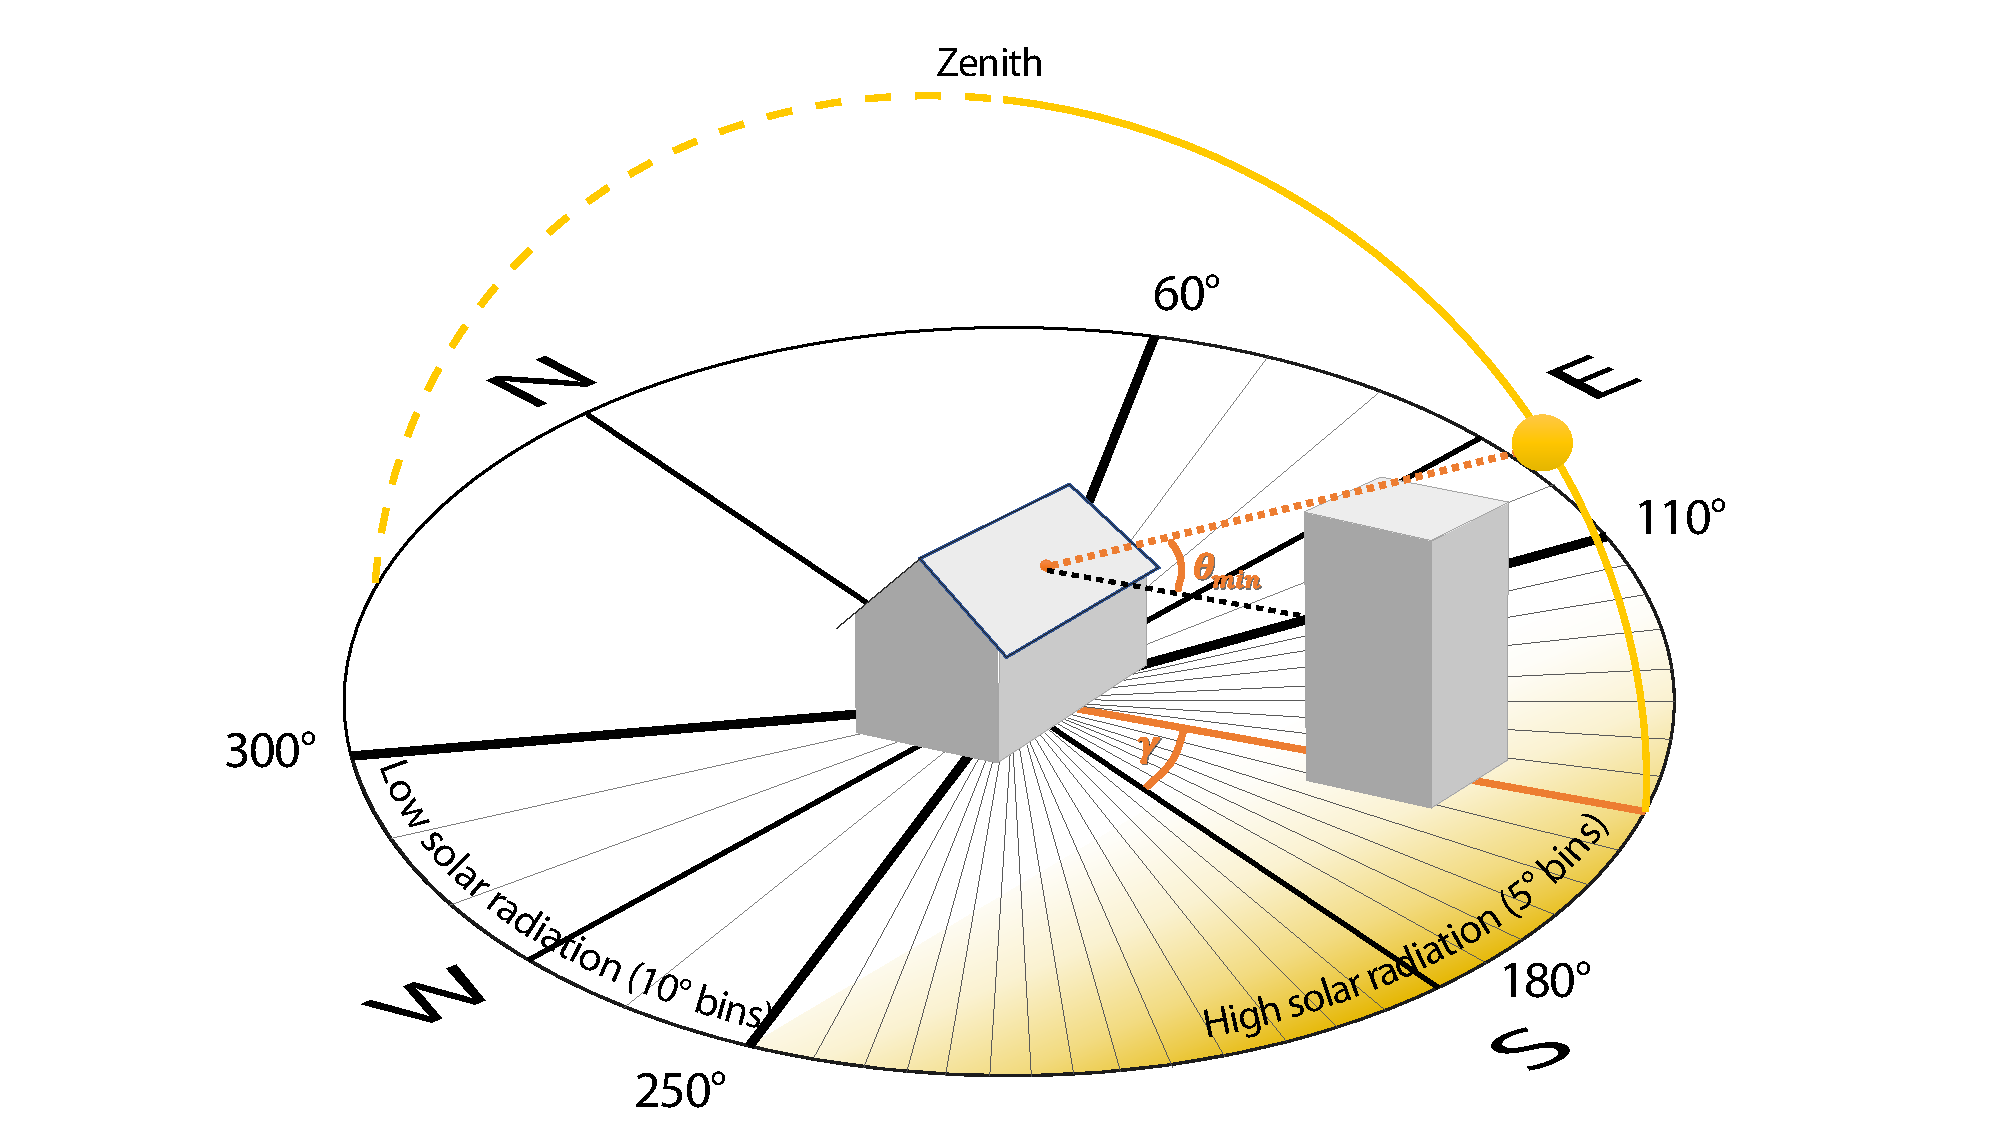
\includegraphics[trim=100 0 130 0, clip, width=.9\linewidth]{Figs/horizon.pdf}  
		\subcaption{}
        \label{figa:horizon_method}
	\end{subfigure}
	\begin{subfigure}[t]{.49\textwidth}
		\centering
		% include second image
		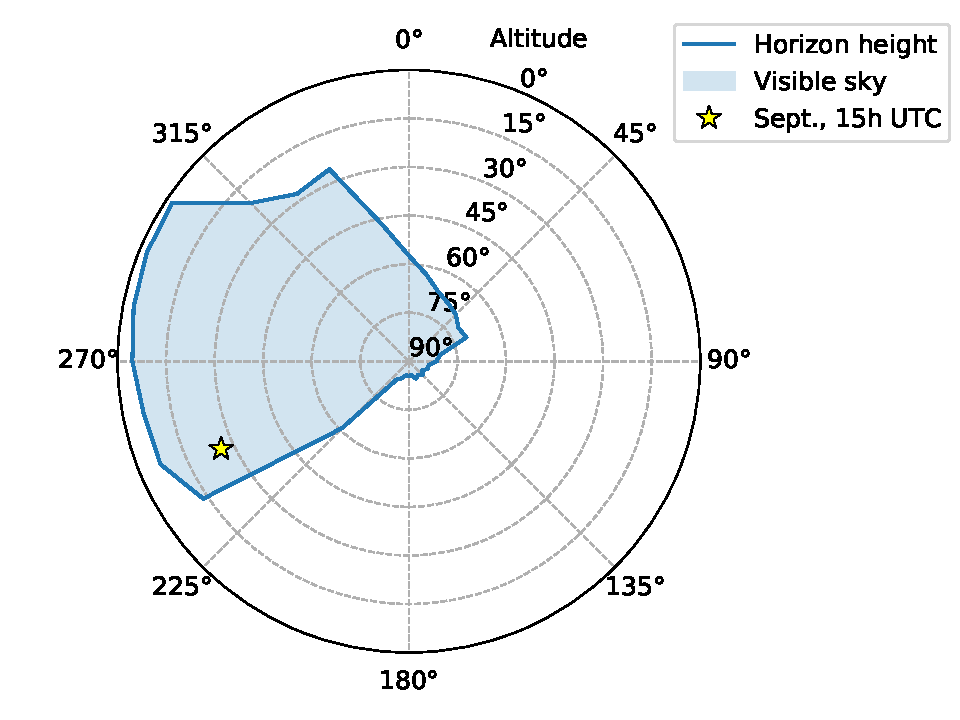
\includegraphics[width=\linewidth]{images/Figs/skyview_point_w_star.pdf}  
		\subcaption{}
		\label{figb:horizon_method}
	\end{subfigure}
	\caption{Horizon modelling for an example roof. (a) Conceptual graph with relevant horizon bins for quantification of shading effects, (b) polar plot of horizon height and visible sky proportion ($\mathit{SVF} = 0.3$), with an example sun position for Switzerland (September, 15h UTC).}
	\label{fig:horizon_method}
\end{figure}

The computation of shading effects and the SVF follow a common 3D modelling approach, known as shadow casting \cite{levinson_solar_2009,desthieux_solar_2018}, ray tracing \cite{jakubiec_method_2013} or viewshed computation \cite{nguyen_incorporating_2012}. 
As shown conceptually in Fig.~\ref{figa:horizon_method}, a 3D model of the environment is used to obtain the horizon height for each aspect angle. 
%
This horizon height ($\theta_\mathit{min}$ in Fig.~\ref{figa:horizon_method}) describes the visible proportion of the sky for a specific aspect angle ($\gamma$ in Fig.~\ref{figa:horizon_method}), and may also be interpreted as the minimum sun elevation angle required to illuminate a given point. 
%
The horizon height for all aspect angles can be visualised as a polar plot, from which the SVF is derived as the visible sky fraction (Fig.~\ref{figb:horizon_method}). The polar plot further indicates whether the given point is shaded during a particular hour of the year based on the sun position (see star in Fig.~\ref{figb:horizon_method}).

\begin{figure}[tb!]
	\centering
	\begin{subfigure}{.49\textwidth}
		\centering
		% include second image
		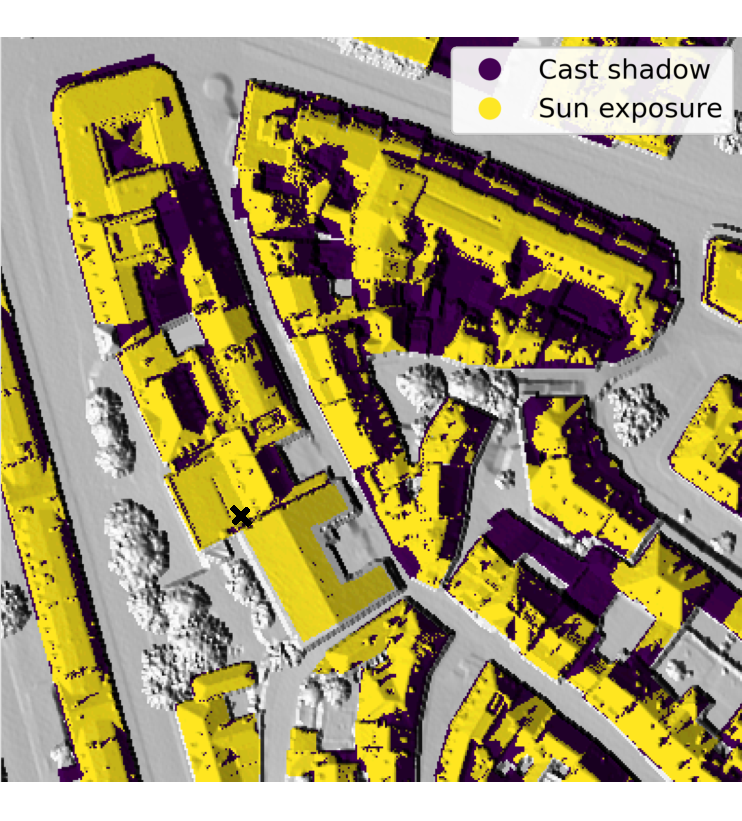
\includegraphics[height=.9\linewidth]{images/Figs/demo_vis_09_15h_w_cross.pdf}  
		\subcaption{}
        	\label{figa:raster_svf_ssh}
	\end{subfigure}
	\begin{subfigure}{.49\textwidth}
		\centering
		% include second image
		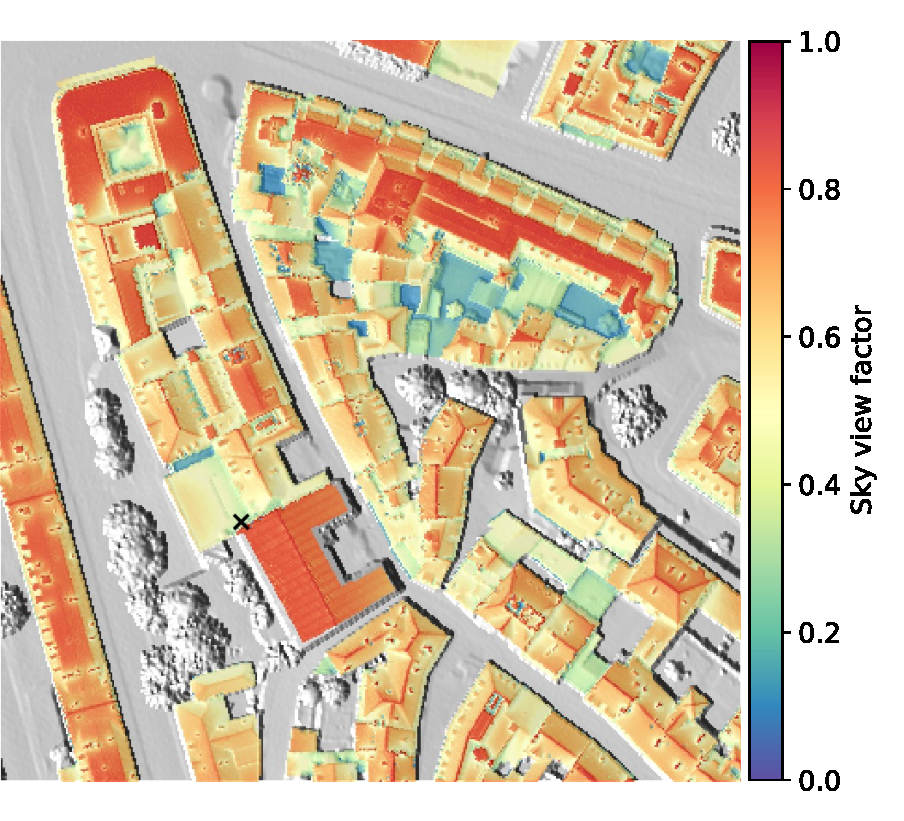
\includegraphics[height=.9\linewidth]{images/Figs/svf_w_legend.pdf}  
		\subcaption{}
        	\label{figb:raster_svf_ssh}
	\end{subfigure}
	\caption{Raster-based (a) cast shadows for one example hour (15h UTC in September, see star in Fig.\ref{figb:horizon_method}) and (b) sky view factor for an area of $200\times200$ m$^2$ in Geneva, Switzerland. The cross on the figures shows the point for which the horizon height is shown in Fig.\ref{figb:horizon_method}.}
	\label{fig:raster_svf_ssh}
\end{figure}

While fisheye images \cite{calcabrini_simplified_2019} or LiDaR point clouds \cite{bill_3d_2016,jakubiec_method_2013} may be used for horizon computations, DEMs are by far the most widely used input data, as they enable the computation of horizon heights for an entire region \cite{suri_new_2004}.
Using a DEM to compute the horizon heights yields a set of raster maps, one for each azimuth angle.
From these, maps of cast shadows (Fig.~\ref{figa:raster_svf_ssh}) can be computed for any sun position, by selecting the horizon map corresponding to the sun azimuth angle and applying a binary filter to the raster values, setting all values below the sun altitude to 1 (sun exposure) and all values above the sun altitude to 0 (cast shadow).
%
The SVF is obtained from a combination of the same set of horizon maps, yielding an SVF for each pixel (Fig.~\ref{figb:raster_svf_ssh}). The SVF is independent of the sun position and hence constant with time. 

While some studies compute PV potential at the level of individual pixels \cite{buffat_scalable_2018,ramirez_camargo_spatio-temporal_2015}, the results are often aggregated per building or roof surface \cite{assouline_quantifying_2017,assouline_large-scale_2018,klauser_solarpotentialanalyse_2016}. To aggregate shading effects or the sky view factor per roof, existing methods use 2D building or roof geometries, which are geospatially intersected with the raster maps to average all pixels within a given roof/building. This geospatial overlay further reduces the data storage requirements for the maps of shading and SVF, as all non-relevant areas for rooftop RPV potential are excluded.

In this work, we use the shadow casting and SVF computation method as detailed above. We use the open-source GRASS-GIS computational engine, which supports the computation of horizon heights \cite{suri_new_2004} and the sky view factor \cite{zaksek_sky-view_2011} and which is used in several of the reviewed studies \cite{ramirez_camargo_spatio-temporal_2015,nguyen_incorporating_2012,buffat_scalable_2018}. 
Further details regarding the implementation of the computation of shading effects and the SVF for scalability to the Swiss national scale are provided Appendix~\ref{app:shade}.

\begin{comment}
\subsection{Solar thermal heat generation}

The computation of the technical potential of a solar thermal collector is more complex to compute, as the solar thermal collector is typically coupled with a heat pump and a hot water tank. In the thermal application, the temperature of the collector and the ambience also play a larger role. Some studies still consider a constant efficiency value [27], while several studies suggest to consider temperature and incident irradiance [11], [28], [29].
\end{comment}

\subsubsection{Available area for solar panel installation}
%% ADD FIGURE??

Based on the an early study of RPV potential in Europe \cite{iea_potential_2002}, we identify three factors of the rooftop available area that are accounted for to different extents in the literature, namely (i) the total roof area, (ii) the roof utilisation and (iii) the roof exposure or suitability. 
\\

\textbf{Total roof area.} For the estimation of RPV yield, three characteristics of the roof areas are relevant: the roof geometries, the tilt angle and the aspect angle. Geospatial datasets containing these characteristics are already available in some countries such as Switzerland (see Chapter~\ref{data_geometry}).
If no rooftop data is available, rooftop tilt and aspect angles can be derived from a DEM \cite{ramirez_camargo_spatio-temporal_2015} or LiDaR point cloud \cite{buffat_feature-aware_2016,nguyen_incorporating_2012}.
To classify different roof surfaces, these may be combined with building geometries from Open Street Map (OSM) or local survey data \cite{ramirez_camargo_spatio-temporal_2015}.
\citet{mohajeri_city-scale_2018} propose an ML approach to classify roof shapes based on DEM-derived features aggregated within building geometries.
In absence of building geometries, aerial images may be segmented using GIS-based featture extraction \cite{wiginton_quantifying_2010} or Convolutional Neural Networks (CNN) \cite{zhao_object-based_2017} to detect building footprints.

Even without DEM, LiDaR or other 3D building data, the roof aspect angle can be approximated from the building geometry as the angle normal to the roof ridge line or building wall \cite{mainzer_assessment_2017}. 
Aerial images themselves however do not provide any information on the roof tilt angle.
% Without any DEM, LiDaR or other 3D building data, no information on tilt and aspect angles of rooftops can be derived. 
For the purpose of large-scale RPV studies, \citet{mainzer_assessment_2017} thus suggest to use a statistical approach, which randomly assigns tilt angles using a normal distribution fitted for a set of buildings with available roof tilt data for Germany.

\textbf{Roof utilisation} refers here to any factors reducing the available area for solar panel installation due to alternative uses. Using the definition by the \citet{iea_potential_2002} ("architectural suitability"), this includes (i) any obstructing objects on roofs, such as fixed superstructures (e.g. dormers, chimneys, elevators), roof-mounted structures (e.g. HVAC equipment) and windows, (ii) surfaces used for other purposes, such as roof terraces or gardens, (iii) protected roofs, and (iv) shaded areas. As quantifying these factors requires the availability of high-resolution 3D building data or aerial imagery, many studies employ constant value methods \cite{assouline_estimation_2017}, which assume a constant ratio of available area. These constant values may vary for different building types and/or roof sizes \cite{wegertseder_combining_2016,portmann_sonnendach.ch:_2016,wiginton_quantifying_2010}. 

Obstructing objects on roofs are most easily identified and removed from the total roof area using manual labelling of aerial images, as performed for example in \cite{ordonez_analysis_2010,strzalka_large_2012}. This approach is only feasible for a small sample size \cite{ordonez_analysis_2010}.
At larger scale, high-resolution 3D building models, such as CityGML datasets with an LOD~4 standard, have been used to exclude superstructures from rooftops \cite{assouline_quantifying_2017}.
These 3D building models however do not include rooftop-mounted structures or windows.
Such objects can only be automatically detected using image processing approaches, as proposed by \citet{mainzer_assessment_2017} who use an edge-detection algorithm to identify obstructing objects.
\citet{castello_deep_2019} have used a CNN algorithm to detect existing PV panels on building rooftops, which may be transferable to the detection of available area for RPV installation.

Going beyond the detection of obstructing objects, several studies assess the area that may be covered by PV panels, by virtually installing PV panels (rectangular polygons) on the geometries of the available area \cite{ordonez_analysis_2010,mainzer_assessment_2017,assouline_large-scale_2018}. 
This virtual panel placement accounts for the impact of rooftop geometries and the location of existing superstructures on the potential number of PV panels and allows to simulate different arrangements of PV panels, for example on flat roofs \cite{ordonez_analysis_2010}.

In contrast to obstructing objects, alternative uses of the roof surfaces and potential protection of buildings cannot be derived from 3D models. Aerial imagery may provide some information to this aim, as terraces for example may contain some non-fixed objects such as tables and chairs which could be classified as unsuitable for PV installation by an automatic image processing method. However, no current methodology follows this approach. 
Protected roofs may be identified by local inventories of protected buildings. 
Alternatively, \citet{florio_assessing_2018} propose a method to quantify rooftop visibility in urban settings.
Shaded areas, which may be obtained from the shadow casting approach described above, are excluded as part of the roof utilisation for example in \cite{singh_estimation_2015,hong_development_2017}.

\textbf{Roof exposure/suitability.} In addition to roof utilisation, large-scale studies of RPV potential exclude areas which are expected to provide a low electricity yield. This roof suitability may be based on a low solar irradiation (e.g. $< 1000$ kWh/m$^2$ \cite{buffat_scalable_2018,portmann_sonnendach.ch:_2016,desthieux_solar_2018}), on the roof aspect (e.g. $\leq 90$° from south \cite{assouline_quantifying_2017,assouline_large-scale_2018,nguyen_incorporating_2012}) or on the roof tilt (e.g. $\leq 60$> \cite{jakubiec_method_2013}).
Additionally, large-scale RPV potential studies frequently exclude small areas, as these are unlikely to be economically feasible. Minimum roof area thresholds in the literature range from 8 m$^2$ \cite{assouline_large-scale_2018} to 33 m$^2$\cite{hong_development_2017}.

\begin{comment}
% For individual roofs, panels can be custom-fitted based on aerial photographs ~\cite{ordonez_analysis_2010} to realistically estimate the maximum available area, taking into account the rooftop geometry as well as any obstructing objects inhibiting the placement of solar panels (roof superstructures).
% Custom-fitting however is not scalable to entire cities or regions, requiring either image processing \cite{mainzer_assessment_2017} or high-resolution 3D building models \cite{engel_effiziente_nodate} for a detailed estimation of the available area.
% As the required input data is not available for many study areas and the computational time for these methods may be prohibitively high, approximative approaches are widely used in the literature.
These range from using standard tabulated factors based on expert opinions [26], statistical methods [7] and extrapolation techniques based on Machine Learning [3]. Assouline et al. [14] provide a detailed analysis of these methods. 

Thus, many studies employ constant value methods \cite{assouline_estimation_2017}, which assume a constant ratio of available area. 
These ratios may be formulated with reference to territorial areas or population count \cite{izquierdo_method_2008,iea_potential_2002,wiginton_quantifying_2010,bodis_high-resolution_2019}, based on building prototypes \cite{wegertseder_combining_2016} or formulated as a constant fraction of individual roofs~\cite{portmann_sonnendach.ch:_2016}. 
In studies where detailed roof data is available through building cadastres 
Full rooftops \cite{bodis_high-resolution_2019}, rooftop avail area fraction ()

The geospatial algorithm is used to virtually install PV panels on the tilted roofs by projecting rectangular polygons onto these surfaces, as shown in Fig.~\ref{fig:panels}c. 
The starting point for this process are the roof polygons and superstructures (Fig.~\ref{fig:panels}a). Panels are installed on the grey areas in Fig~\ref{fig:panels}b, after superstructures (if applicable) and a buffer of 40cm are removed from the polygons~\cite{assouline_large-scale_2018}. The panels are installed in adjacent rows along the roof aspect, starting from the bottom left corner, as described in Algorithm \ref{alg:panels}. It is implemented using the python \texttt{geopandas} library \cite{kelsey_jordahl_geopandas/geopandas:_2019}.

Virtual PV panels were placed in both horizontal and vertical alignments, as no alignment has technical advantages over the other and both are widespread. The alignment that allows the higher number of panels to be installed on each roof is selected as final panel alignment. 
\end{comment}

\section{Shallow geothermal energy}
\label{geo_method}

As discussed in Section ~\ref{REN_CH}, ground-source heat pumps (GSHPs) using vertical closed-loop borehole heat exchangers (BHEs) are by far the most widely used technology to extract shallow geothermal energy in Switzerland \cite{blum_statistik_2016}.
%
Focusing on closed-loop BHEs, this section reviews state-of-the-art analytical models to assess the technical geothermal potential of shallow GSHPs. The technical potential is hereby defined as the heat energy that may be annually extracted from a field of BHEs by a GSHP system ($Q_{GSHP}$), which is computed as (cf. \cite{pahud_geothermal_2002}):

\begin{equation}
\label{eq:Q_field_method}
    Q_\mathit{GSHP}=q_\mathit{max} \times t_{op} \times H \times N_\mathit{BHE}
\end{equation}

where $q_\mathit{max}$ is the heat extraction rate from the boreholes (in W/m), $t_{op}$ is the operating time of the system (in h), $H$ is the borehole depth (in m) and $ N_\mathit{BHE}$ is the number of installed BHEs.

To estimate the technical potential, the following factors must be taken into account: 
(i) The depletion of the ground when boreholes are placed too close to each other or too much heat is extracted; (ii) the sizing, geometry and material of the BHE tubes; (iii) the efficiency of the heat pumps that transfer the extracted heat to domestic heating and hot water applications \cite{bayer_geothermal_2019}. 
% The interaction of these components is a dynamical process that changes over time, which is described by the thermal response of the BHEs.

\begin{figure}[bt]
    \centering
    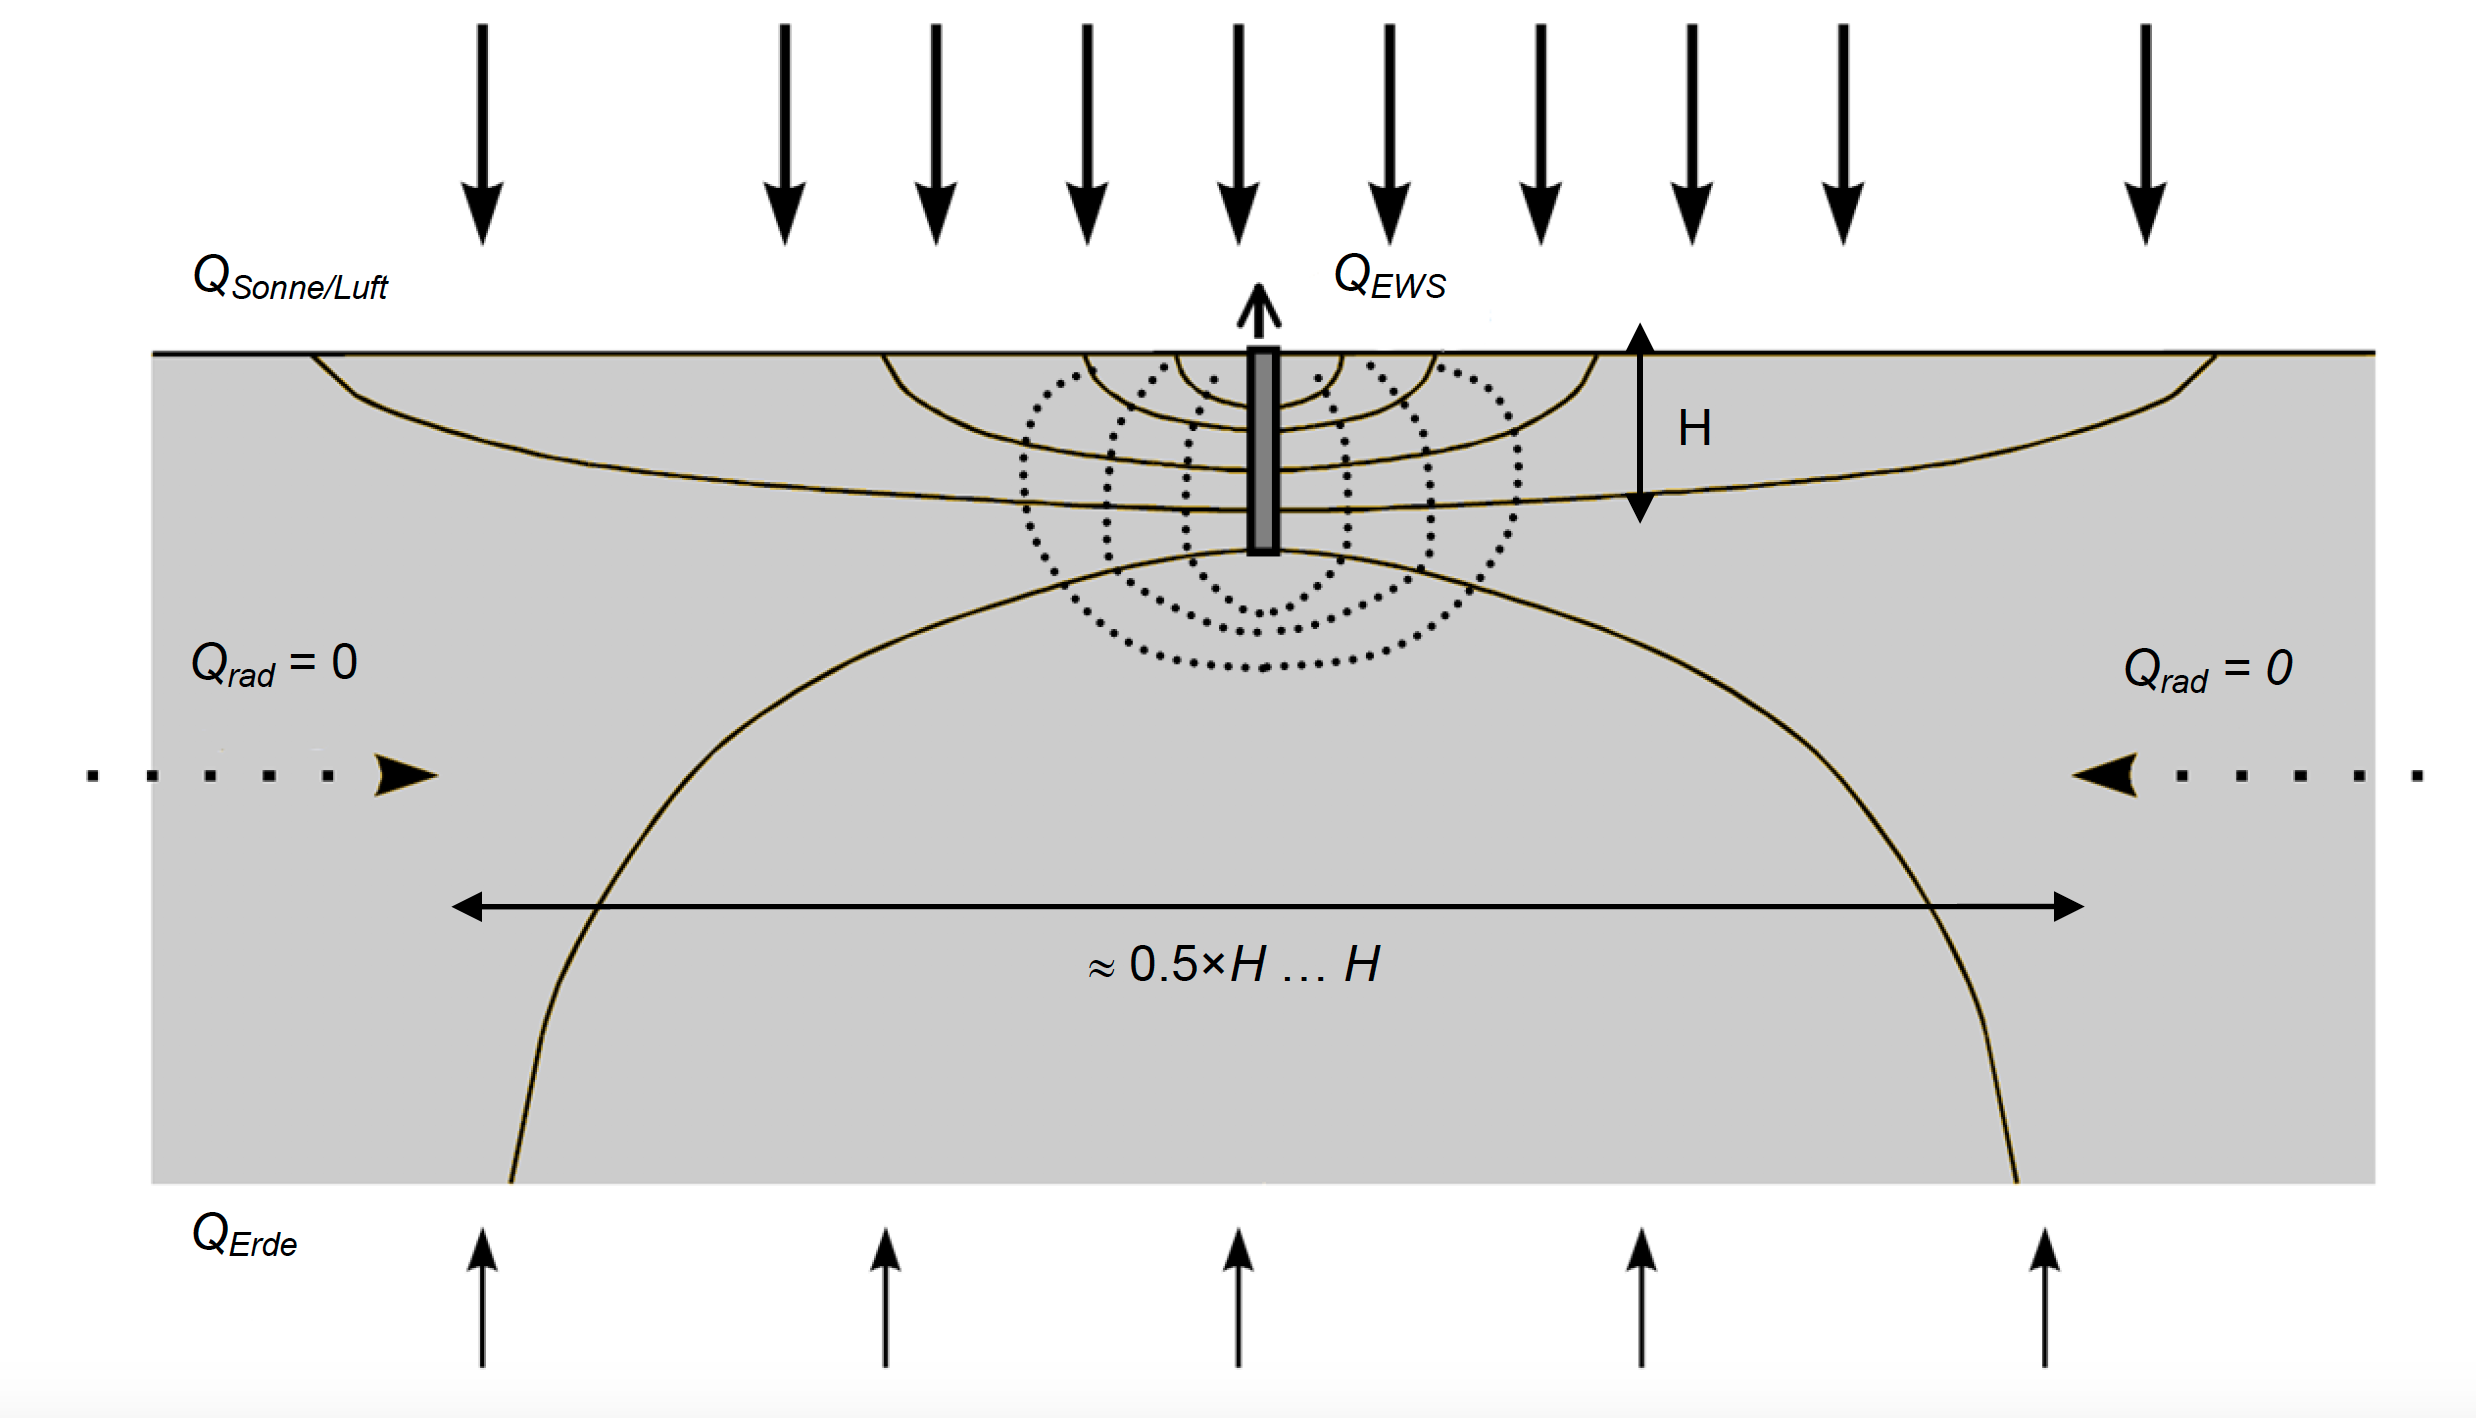
\includegraphics[width=0.7\linewidth]{Figs/BHE_layout.png}
    \caption[Single BHE installation and its effects on the temperature in the ground.]{Single BHE installation and its effects on the temperature in the ground. The arrows on the top indicate the natural heat flux from the environment, those on the bottom indicate the geothermal heat flux. The dashed lines are isothermal lines, while the continuous lines represent the heat flow in the stationary state. Source: \citet{wagner_erdsondenpotenzial_2014}}
    \label{fig:BHE}
\end{figure}

The depletion of the ground is driven by changes in the subsurface temperature, which occur when heat is extracted (or injected) at a faster rate than it is regenerated from the natural heat flux. This heat flux is caused by the heat in the earth's core (geothermal heat flux) and by the heat in the ambient air, as shown in Fig.~\ref{fig:BHE} \cite{wagner_erdsondenpotenzial_2014}.
As heat is extracted from the ground, so-called \textit{thermal plumes} are formed around the BHE (dashed lines in Fig.~\ref{fig:BHE}) \cite{alcaraz_t-i-ger_2017}. Their magnitude and extent depends on the borehole design, particularly the depth and heat extraction rate, as well as on the thermal properties of the ground.
%
When boreholes are spaced too close to each other, thermal plumes may overlap, which causes \textit{thermal interference} between these boreholes and leads to an increased cooling of the subsurface. In this work, quantifying the thermal interference is of high importance, as thermal interference significantly reduces the potential borehole installation density \cite{bayer_geothermal_2019,miglani_methodology_2018}.

Thermal interference between boreholes is assessed in the literature based on an analytical model, developed by \citet{eskilson_thermal_1987}, which simulates the thermodynamic behaviour of BHEs based on the thermal ground properties as well as the sizing, geometry and material of the BHEs.
%  (e.g. \cite{miglani_methodology_2018,rivera_increased_2017,bayer_strategic_2014})
%
To formulate a technical potential for closed-loop GSHPs, related studies (e.g. \cite{miglani_methodology_2018,rivera_increased_2017,schiel_gis-based_2016,viesi_gis-supported_2018,casasso_g.pot:_2016,perego_techno-economic_2019}) combine the this analytical model with norms for the current BHE design practice, using primarily the geothermal norms of the Association of German Engineers (VDI) \cite{vdi_vdi_2019} and the Swiss Society of Engineers and Architects (SIA) \cite{sia_sondes_2010}.
The parameters required for the analytical model and their values given by the SIA norm (relevant for Switzerland) will be introduced in Section~\ref{geo_params}.

Both the VDI and SIA norms require the BHEs to be designed and operated such that the mean temperature of the borehole fluid ($T_{mf}$) never drops below its freezing temperature ($T_\mathit{mf,min}=-1.5$ °C \cite{sia_sondes_2010}), such that \cite{sia_sondes_2010,vdi_vdi_2019}:

\begin{equation}
\label{eq:T_mf_min}
T_{mf} \geq T_\mathit{mf,min} = -1.5 \text{°C}
\end{equation}

The variables in Eq.~\ref{eq:Q_field_method} ($q_\mathit{max}$, $t_{op}$, $H$, $N_\mathit{BHE}$) must hence be chosen such as to fulfil this technical requirement.
%
The relationship between these variables and the $T_{mf}$ is expressed by the borehole \textit{temperature profile}, which describes the temperature changes inside and around a BHE.
A general model of this temperature profile, proposed by \citet{claesson_conductive_1988}, is introduced in Section~\ref{model_intro}, while Section~\ref{geo_models} details the analytical formulas used to estimate the thermodynamic processes in the ground.

While heat extraction is the dominant mode of operation of GSHPs in Europe \cite{lund_direct_2020}, GSHPs can also be used for heat injection, for example for space cooling applications \cite{kavanaugh_geothermal_2014}, whereby the same physical principles (Sections ~\ref{model_intro} and \ref{geo_models}) apply.
As heat injection is not addressed in the SIA or VDI norms, studies addressing the potential of GSHPs for heat injection use the standards of the American Society of Heating, Refrigerating and Air-Conditioning Engineers (ASHRAE) \cite{kavanaugh_geothermal_2014} for borehole sizing \cite{aditya_environmental_2020,miglani_methodology_2018,michopoulos_potential_2011} . For cooling-dominated systems, the temperature requirement from Eq.~\ref{eq:T_mf_min} is inverted, limiting the maximum fluid temperature $T_\mathit{mf,max}$:

\begin{equation}
\label{eq:T_mf_max}
T_{mf} \leq T_\mathit{mf,max}
\end{equation}

In addition to the BHEs, a GSHP system contains a heat pump (HP), which is used to transfer the heat extracted from the ground to the building heating or cooling systems (see Fig. \ref{fig:HP}).
%, as these typically require different temperatures than those provided by the BHE. 
HPs have a high system efficiency, expressed through the coefficient of performance (COP), making GSHPs a very energy efficient technology for building thermal energy supply. Based on the COP, the heat supplied to the building heating ($Q_\mathit{heat}$) and cooling ($Q_\mathit{cool}$) systems is computed as \cite{kavanaugh_geothermal_2014}: 

\begin{equation}
\label{eq:COP_heat}
Q_\mathit{heat}=Q_\mathit{extr}\ \frac{COP_\mathit{heat}}{\left(COP_\mathit{heat}-1\right)}
\end{equation}

\begin{equation}
\label{eq:COP_cool}
Q_\mathit{cool}=Q_\mathit{inj}\ \frac{COP_\mathit{cool}}{\left(COP_\mathit{cool}+1\right)}
\end{equation}

where $Q_\mathit{extr}$ and $Q_\mathit{inj}$ are the extracted and injected heat from/to the BHEs and $COP_\mathit{heat}$/$COP_\mathit{cool}$ are the COPs for heating and cooling, respectively. In neighbourhood or regional-scale studies of technical GSHP potential, constant values are often used for the COP \cite{miglani_methodology_2018,schiel_gis-based_2016,perego_techno-economic_2019}, while studies at building scale typically model the COP as a function of temperature \cite{fraga_heat_2018,liu_feasibility_2017,stene_residential_2005}.

\begin{figure}[bt]
    \centering
    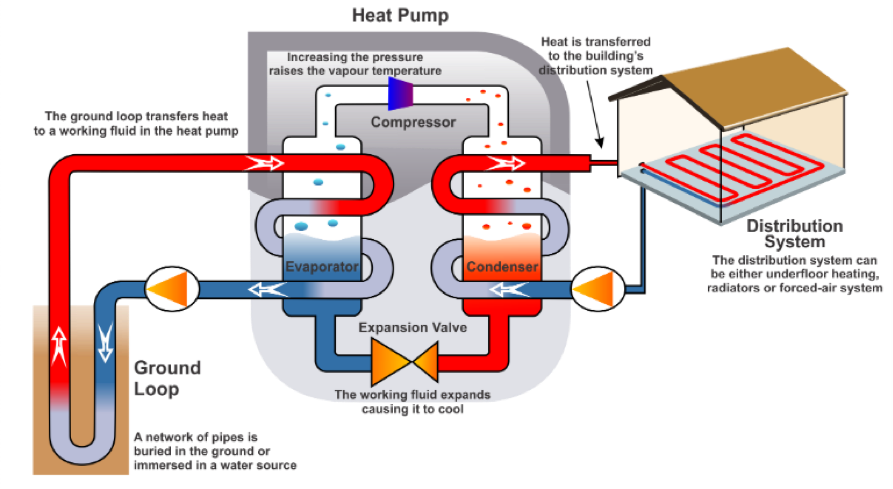
\includegraphics[width=0.7\linewidth]{images/Figs/GSHP.png}
    \caption{Working principle of a GSHP in heating cycle. Cold air is moved from the house to the heat pump, where it is heated from the compressed heat extracted from the ground. The ground loop liquid is cooled and transported back to the ground, where it is again heated \cite{gns_science_n.z._geothermal_2016}.}
    \label{fig:HP}
\end{figure}

\subsection{Parameters}
\label{geo_params}
The parameters involved in the modelling of the thermodynamic behaviour of borehole heat exchangers can be divided into three groups: 

\begin{enumerate}
\item \textbf{Physical parameters} are given by the geological and hydrological conditions of the ground, and are the subject of various large-scale studies \cite{signorelli_regional_2004,majorowicz_estimation_2009,tian_improved_2020}. Seasonal temperature variations in the ground are neglected, as boreholes typically have a depth $> 50$ m, which is beyond the penetration depth of seasonal variations in the ground \cite{stauffer_thermal_2013}.

\item \textbf{Technical parameters} are derived from the materials and the technology of the BHEs. In this work, we use constant values based on the related literature and do not address the impact of their variation on the BHE potential.

\item \textbf{Design parameters} are related to the sizing of the BHEs and the borehole fields, in order to estimate a technical potential of GSHPs. These parameters and the impact of their variation on the GSHP potential are the main subject of this section. 
\end{enumerate}

We refer to $z$ (in m) for the depth in the ground, $r$ (in m) for the radial distance to the center of a BHE, $t$ (in hours or years) for the time and $T$ (in °C or K) for the temperature. 

\begin{table}[b]
\footnotesize
\caption{Physical parameters. Norm values and ranges for Switzerland are obtained from \citep{sia_sondes_2010}.}
\label{tab:phys_params}

\centering
\begin{tabular}{lllll}
\hline
\textbf{Symbol}             & \textbf{Unit} & \textbf{Description}           & \textbf{Formula}                                      & \textbf{Norm value / range (CH)} \\ \hline
$\lambda$                   & W/mK        & Thermal conductivity           &                                                       & $1-4$ (Plateau: $2-3$)           \\
$\alpha$                    & m$^2$/s       & Thermal diffusivity            & $\alpha = \frac{\lambda}{\rho C}$                     & $0.9-1.4 \times 10^{-6}$         \\
$\rho C$                    & MJ/m$^3$K      & Volumetric heat capacity       &                                                       & $1.2-3.5$ (Plateau: $2-2.5$)     \\ \hline
$T_g(z)$                    & °C    & Undisturbed ground temperature &                                                       & \textit{Norm}: 10                         \\
$\frac{\Delta T}{\Delta z}$ & K/m         & Temperature gradient           & $T_g(z) = T_0 + z * \frac{\Delta T}{\Delta z} $       & Plateau: 0.03, Alps: 0.025       \\
$T_0$                       & °C    & Surface temperature            &                                                       & \textit{Norm}: 8.5                        \\ \hline
$\dot{q}_{g}$               & mW/m$^2$      & Geothermal heat flow           & $\dot{q}_{g} = \lambda * \frac{\Delta T}{\Delta z}$   & $40-170$                         \\ \hline
\end{tabular}
\end{table}

\textbf{Physical parameters}. The physical parameters are listed in Table~\ref{tab:phys_params}. The \textit{thermal conductivity} $\lambda$ and \textit{thermal diffusivity} $\alpha$ are used in the analytical models. However, the geological properties of different types of rocks are typically provided as $\lambda$ and the \textit{volumetric heat capacity} $\rho C$. From these parameters, the thermal diffusivity is computed as \cite{pahud_geothermal_2002}:

\begin{equation}
\label{eq:alpha}
    \alpha = \frac{\lambda}{\rho C}
\end{equation}

In the literature, the values for $\rho C$ and $\lambda$ are either derived from measurement data and interpolated using geostatistical kriging \cite{tian_improved_2020,munoz_estimating_2015} or Machine Learning~\cite{assouline_machine_2019}, obtained from 3D underground models \cite{garcia-gil_gis-supported_2015,groupe_de_travail_pgg_evaluation_2011} or, most frequently, mapped from tabulated values in the literature based on the present rock types~\cite{perego_techno-economic_2019,galgaro_empirical_2015,casasso_g.pot:_2016,gemelli_gis-based_2011}. An overview of typical thermal conductivity and heat capacity values for rock types found in Switzerland are provided in the SIA norm \cite{sia_sondes_2010} and by \cite{pahud_geothermal_2002}.
\\

If hydro-geological data is available, the thermal conductivity can be adjusted to account for conductive heat transfer due to groundwater movement \cite{viesi_gis-supported_2018,assouline_machine_2019}, using the ground saturation level and the darcy velocity as input \cite{viesi_gis-supported_2018}. 
Advective heat transfer is neglected in the model proposed by \citet{eskilson_thermal_1987}.
Analytical models accounting for advective heat transfer have been used for example in \cite{garcia-gil_gis-supported_2015,alcaraz_advection_2016,alcaraz_t-i-ger_2017,attard_novel_2020}.
As the hyrdo-geological input data required for these advective-conductive models is not available at the regional scale for Switzerland, this thesis focuses on the conductive heat transfer model \cite{claesson_conductive_1988}. A similar approximation is applied in most related regional-scale studies, including \cite{perego_techno-economic_2019,galgaro_empirical_2015,casasso_g.pot:_2016,rivera_increased_2017,schiel_gis-based_2016}.

Another important physical parameter is the \textit{undisturbed ground temperature} $T_g(z)$. In particular, the temperature at half of the borehole depth ($z = H/2$) is of interest. If no data is available for estimating $T_g$ directly, it can be extrapolated from the \textit{surface temperature} $T_0$ and the \textit{temperature gradient} $\Delta T/\Delta z$: 

\begin{equation}
\label{eq:Tg}
    T_g(z) = T_0 + z * \frac{\Delta T}{\Delta z}
\end{equation}

\begin{figure}
    \centering
    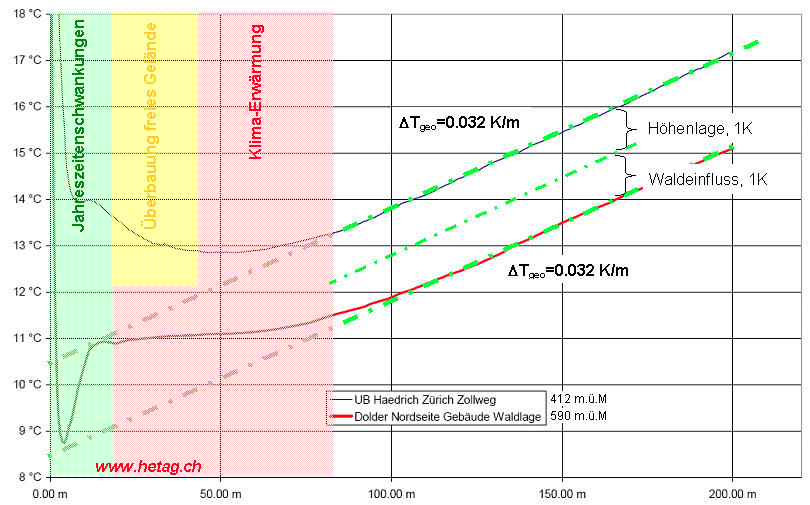
\includegraphics[width=0.6\linewidth]{Figs/ground_temperature.png}
    \caption[Example for the variation in ground temperature for two measurements of ground temperature in Zürich.]{Example for the variation in ground temperature for two measurements of ground temperature in Zürich, showing the influence of altitude (black line) and additional surface heating through the presence of forests (red line). Source: \citet{huber_bodentemperaturen_2014}.}
    \label{fig:T_ground}
\end{figure}

The $T_0$ can be either interpolated based on measurements of the near-surface ground temperature \cite{assouline_machine_2019} or derived from measurements of the ambient temperature ($T_\mathit{amb}$). An analysis of different methods to determine $T_0$ is performed in \citep{signorelli_geoscientific_2004}. In the SIA norm, surface temperatures are  approximated from the mean annual $T_\mathit{amb}$ by adding an altitude-dependent term \cite{sia_sondes_2010}. As the actual $T_0$ may deviate from the approximated value (see Fig.~\ref{fig:T_ground} for an example), the SIA norm instructs the addition of a tolerance ($\Delta T$) of $- 1$ K heating for  $+1$ K for cooling.

While not being directly used in the analytical model of GSHPs, the (undisturbed) \textit{geothermal heat flow} $\dot{q}_{g}$ plays an important role in the quantification of geothermal resources, as it characterises the natural heat flow in the ground. It is given by \cite{huber_bodentemperaturen_2014}:

\begin{equation}
    \dot{q}_{g} = \lambda * \frac{\Delta T}{\Delta z}
\end{equation}

The geothermal heat flow is approximately constant across the outer crust of the earth, but may vary in mountain terrain \citep{huber_bodentemperaturen_2014}. The relationship may further be used to compute $\lambda$ or $ \frac{\Delta T}{\Delta z}$ if other data is unavailable.

\begin{figure}[b]
    \centering
    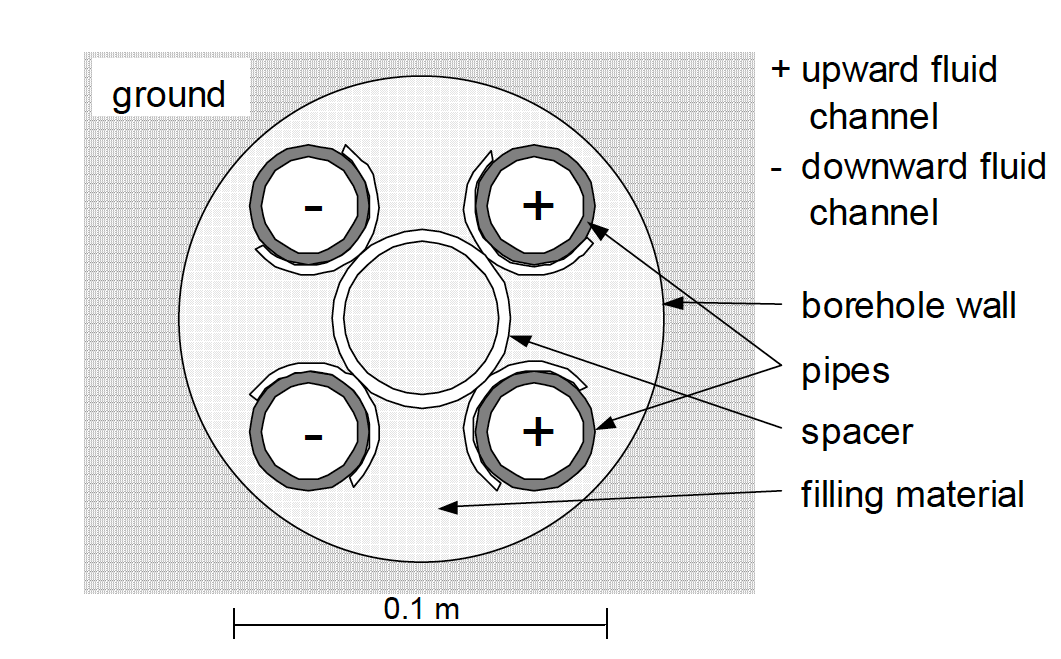
\includegraphics[width=0.6\linewidth]{Figs/BHE_tech.png}
    \caption[Cross-section of a duplex BHE layout.]{Cross-section of a duplex BHE layout \citep{pahud_geothermal_2002}.}
    \label{fig:BHE_cross-sec}
\end{figure}

\textbf{Technical parameters}. The technical parameters required to determine the technical geothermal potential are set as constant values in the literature (e.g. \cite{miglani_methodology_2018,rivera_increased_2017,zhang_critical_2017}). The $T_\mathit{mf,min}$ temperature is set in most reviewed studies to $-1.5^\circ C$ \citet{sia_sondes_2010}.
For $T_\mathit{mf,max}$, no unique value exists across the literature. Instead, \citet{kavanaugh_geothermal_2014} suggest to choose a $T_\mathit{mf,max}$ of $11 - 18$ °C above $T_g$.
% \cite{spitler_vertical_2016}.
Quantifying the temperature drop inside the borehole further requires knowledge of the borehole radius ($r_b$) as well as the effective thermal resistance of the borehole ($R_b^*$). A typical layout of a duplex system, the most common form of BHE installations (\cite{sia_sondes_2010}), is shown in Fig.~\ref{fig:BHE_cross-sec}. The thermal resistance is determined by the materials and the geometry of the BHE, which are analysed in detail in \citep{huber_erdwarmesonden_2005}. Table~\ref{tab:tech_design_params} summarises the range of parameters found in the literature and the SIA norm values (if applicable).

\textbf{Design parameters}. Two groups of design parameters are relevant to study the multi-fold effects between the geometry of a BHE field and the temperature in the ground, which is typically assessed after a planning horizon $t_\mathit{dim}$. 
The first group of parameters are related to the borehole geometry. These include the borehole depth ($H$), the horizontal distance between BHEs ($B$) and the distance between the top part of the BHE (where heat is extracted) and the ground surface ($D$). 

A second group of design parameters is related to the heat extraction from the borehole. It includes the heat extraction power ($Q_{HP}$), the maximum heat extraction rate ($q_\mathit{max}$), the operating time ($t_{op}$) and the duration of maximum operation ($t_{peak}$). The heat extraction power is related to the power rating of the heat pump (HP), whose typical values are shown in Table~\ref{tab:tech_design_params}. 
% In a large-scale study, however, $Q_{HP}$ is not a technical parameter, as the number of heat pumps in the system is undefined. 
The heat extraction rate is computed from $Q_{HP}$ and $H$ as given in Table~\ref{tab:tech_design_params}. Nominal curves for $q_\mathit{max}$ as a function of $\lambda$ and $\rho C$, referred to as nominal heat extraction rate $q_{nom}$, are provided in \cite{sia_sondes_2010}. These curves can be approximated as (cf. \cite{sia_sondes_2010}):

\begin{equation}
\label{eq:q_nom}
    q_{nom} \approx \frac{T_g - T_\mathit{mf, min}}{11.5} \ \left( 10.6 \lambda + 11.2 + 2 \left( \frac{\lambda}{\alpha} - 2 \right) \right)
\end{equation}

% If these are used, $Q_{HP}$ needs to be computed by rearranging the equation for $q_\mathit{max}$. 
The operating time indicates the number of hours in which the heat pump is operating (with power $Q_{HP}$). The norm values, used throughout this work, depend on altitude and location \cite{sia_sondes_2010}.
%. It changes with altitude and location, and the nominal values are shown in Fig.~\ref{fig:t_q_norm}b. 
The duration of the peak extraction pulse ($t_\mathit{peak}$) measures the maximum time of non-stop operation of the HP, which impacts the maximum temperature drop in the BHE and is usually taken as 1, 5 or 10 days \cite{pahud_geothermal_2002}.

\begin{table}[t]
\footnotesize
\caption{Technical and design parameters. Norm values are given in \citep{sia_sondes_2010}, while other parameters are obatined from related studies \citep{pahud_geothermal_2002, wagner_erdwarmesonden._2019, claesson_conductive_1988}.}
\centering
\resizebox{\textwidth}{!}{%
\begin{tabular}{lllll}
\hline
\textbf{Symbol} & \textbf{Unit} & \textbf{Description}                   & \textbf{Formula}                                        & \textbf{Norm value / range (CH)} \\ \hline
$T_{f, min}$    & °C   & Minimum mean fluid temperature         & $T_{f} = \frac{T_{in} + T_{out}}{2}$                    & \textit{Norm}: $- 1.5$           \\
$r_b$           & m           & Borehole radius                        &                                                         & $0.055-0.07$                      \\
$R_b^*$         & mK/W        & Effective borehole resistance          &                                                         & $0.08-0.1$                       \\ \hline
$H$             & m           & Borehole depth                         &                                                         & \textit{Norm}: $100$ (mostly $50-200$)          \\
$D$             & m           & Distance between $z=0$ and BHE outlet  &                                                         & $2-5$                              \\
$B$             & m           & Spacing between BHEs                   &                                                         & $>5$ (no effect for B $>$ H)     \\ \hline
$Q_{HP}$        & W           & Heat extraction power during operation &                                                         & $4500-8400$                      \\
$q_\mathit{max}$       & W/m         & Maximum heat extraction rate           & $q_\mathit{max} = \frac{Q_{HP}}{H}$                            & \textit{Norm} ($q_{nom}$): $20-55$           \\
$t_{op}$        & h           & Annual operation time                  &                                                         & \textit{Norm}: $1850$  \\
$t_{seas}$      & years           & Periodicity of seasonal heat extraction  &                                                         & 1                 \\ 
$t_{peak}$      & h           & Duration of maximum extraction pulse   &                                                         & $1 - 10$ days                    \\ 
\hline
$t_\mathit{dim}$       & years           & Planning horizon for dimensioning the BHE   &                                                         & $50$                    \\ 
\hline
\end{tabular}
}
\label{tab:tech_design_params}
\end{table}

\subsection{Temperature profile of a BHE installation}
\label{model_intro}

To quantify the temperature field of a BHE, we distinguish between the processes inside and outside the BHE. The temperature drop inside the BHE, i.e. between the heat carrier fluid at mean temperature $T_f$ and the borehole wall at temperature $T_b$, is a function of the heat extraction rate and the effective thermal resistance of the borehole, such that \citep{claesson_conductive_1988}:

\begin{equation}
\label{eq:T_b}
    T_b(t) - T_f(t) = q_\mathit{max}*R_b^*
\end{equation}


The temperature at the borehole wall $T_b$ differs from the undisturbed ground temperature $T_g$ by a temperature drop $\Delta T_b$. It varies with depth ($z$), so the average value along the borehole may be obtained by numerical integration ($z = \overline{z}$) or, in a simplified way, by taking $z = H/2$. The borehole wall temperature $T_b$, with $r = r_b$, is hence computed as:

\begin{equation}
    T_b(z, t) = T_g(z) - \Delta T_b(z, t)
\end{equation}

\begin{figure}
    \centering
    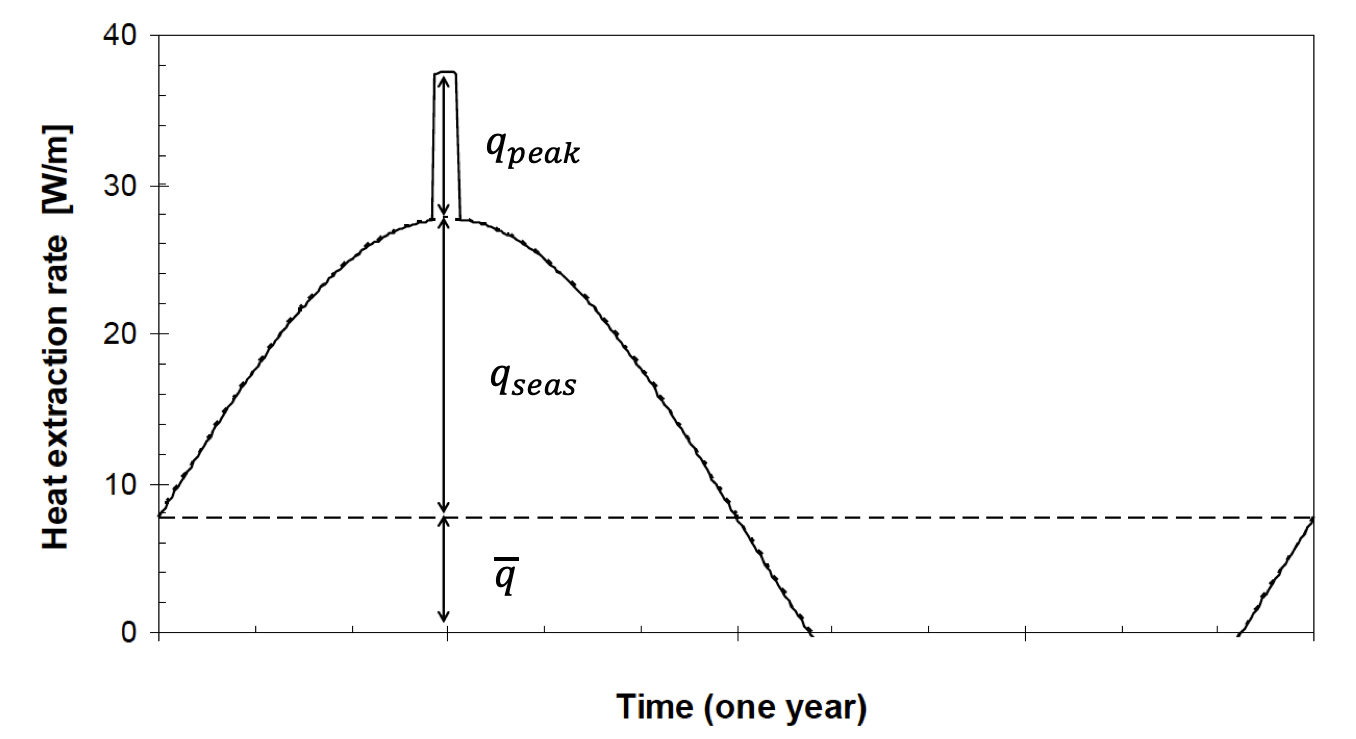
\includegraphics[width=.6\linewidth]{Figs/q_seasonal.png}
    \caption{"Simplified heat extraction rate evolution for a typical year (constant + periodic + pulse)" \citep{pahud_geothermal_2002}.}
    \label{fig:q_seasonal}
\end{figure}

The analytical model proposed by \citet{eskilson_thermal_1987} is based on the principles of temporal and spatial superposition, which assumes that $\Delta T_b$ is the sum of the temperature drops due to heat extraction pulses of different duration and from any neighbouring borehole, whereby boreholes at distances greater than $H/2$ can be neglected \cite{pahud_geothermal_2002}.

The principle of temporal superposition implies that $\Delta T_b(z, t)$ can be modelled as a long-term (\textit{LT}), a seasonal (\textit{seas}) and a short-term (\textit{peak}) component \citep{claesson_conductive_1988}, as shown in Fig.~\ref{fig:q_seasonal}.
%
% A method to model these effects, shown in Fig.~\ref{fig:q_seasonal}, is suggested in  and summarized in \cite{pahud_geothermal_2002}. 
%
Long-term effects are represented by a constant heat extraction rate $\overline{q}$, which is typically assessed for a planning horizon ($t_\mathit{dim}$) of 20 or 50 years \cite{pahud_geothermal_2002,miglani_methodology_2018}. 
Seasonal effects are represented as a sinusoidal heat extraction with peak rate $q_\mathit{seas}$ and period $t_\mathit{seas}$ of 1 year.
% , so that the annual integral is zero.
The peak extraction, which occurs at maximum seasonal extraction, has a duration $t_\mathit{peak}$ (typically 1-10 days). The energy extracted from this pulse is neglected \cite{claesson_conductive_1988}. 
To obtain $\Delta T_b$, each heat extraction rate is multiplied with a respective thermal resistance ($R_{LT},R_\mathit{seas},R_\mathit{peak}$) \cite{claesson_conductive_1988}:

\begin{equation}
\label{eq:dT_b}
    \textstyle \Delta T_b(z, t) = \overline{q} * R_{LT}(z, t) + q_{seas} * R_{seas}(z,t) + q_{peak} * R_{peak}(z, t)
\end{equation}
where
\begin{equation*}
    \overline{q} = \frac{t_{op}}{365*24} * q_\mathit{max}, \quad q_\mathit{seas} = w_\mathit{seas} * q_\mathit{max}, \quad q_\mathit{peak} = q_\mathit{max} - \overline{q} - q_\mathit{seas}
\end{equation*}

and $w_\mathit{seas}$ is the seasonal system load, given as a dimensionless constant.

Equation~\ref{eq:dT_b} can be used to simulate the temperature variation at the borehole wall for any time $t$. 
For GSHP system sizing and to assess the potential long-term heat extraction from the ground, the worst-case $\Delta T_b$ and consequently the lowest $T_{mf}$ (or highest, for heat injection) must be calculated and substituted in Eqs.~\ref{eq:T_mf_min} (heat extraction) or \ref{eq:T_mf_max} (heat injection).
To obtain the $T_{mf}$, the temperature drop along the entire borehole is of interest, denoted as $H$ (the borehole depth).
Using this notation, a combination of Eqs.~\ref{eq:T_b}-\ref{eq:dT_b} gives the following equation for the lowest/highest $T_{mf}$:
\begin{equation}
\label{eq:T_mf}
   T_{mf}(t) =  \textstyle T_g\left(\frac{H}{2}\right) - \overline{q} * R_{LT}(H, t_\mathit{dim}) - q_{seas} * R_{seas}(t_\mathit{seas}) - q_{peak} * R_{peak}(t_\mathit{peak}) - q_\mathit{max}*R_b^*
\end{equation}

For reasons explained in Section~\ref{app:models}, only the $R_{LT}$ is a function of the borehole depth $H$.
This equation is valid for the cases of heat extraction (e.g. space heating) and heat injection (e.g. space cooling). The difference between the two modes of operation is that the heat extraction rates ($q$) are positive for heat extraction and negative for heat injection and that their magnitude may vary depending on the length of the heating/cooling seasons and the respective demand.

The principle of spatial superposition implies that the temperature drops due to the heat extraction from neighbouring BHEs is added to the temperature drop at the borehole wall. 
%
As the seasonal and peak effects are of a short duration and have a penetration radius of less than the minimum borehole distance $B_{min} = 5$m \cite{pahud_geothermal_2002}, the seasonal and peak components of neighboring boreholes hence do not interfere with each other.
%
The long-term temperature drop ($\Delta T_{LT}$), however, may be impacted by surrounding boreholes. Fig.~\ref{fig:T_field} shows the long-term $\Delta T$ for different times, (a) at the borehole wall as a function of $z$ and (b) integrated along $z$ (denoted as $\overline{z}$ in Fig.~\ref{fig:T_field}b) as a function of distance to the borehole. Most of the temperature drop occurs during the first 10 years of operation, while the temperature drop after the planning horizon of 50 years is small.

\begin{figure}
    \centering
    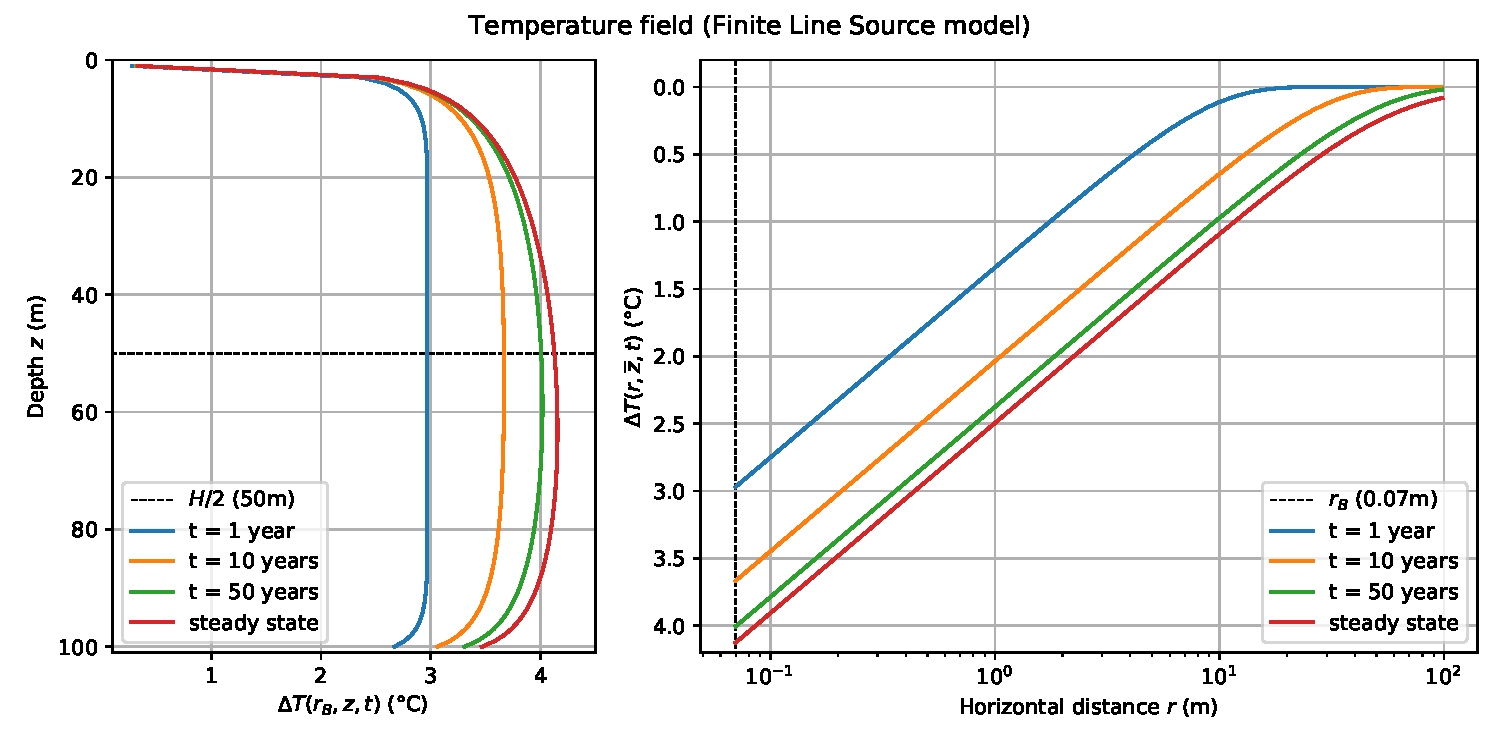
\includegraphics[width=.9\linewidth,trim={0 .6cm 0 .7cm},clip]{Figs/temp_field_FLS.pdf}
    \begin{subfigure}[t]{.42\textwidth}
        \centering
    \subcaption{}
      \label{figa:T_field}
    \end{subfigure}
    \begin{subfigure}[t]{.45\textwidth}
      \centering
        \subcaption{}
      \label{figb:T_field}
    \end{subfigure}
    \caption{a) Long-term variation of the ground temperature at the borehole wall ($\Delta T_{LT}(r_b, z, t)$) as a function of depth ($z$), b) Integration of $\Delta T_{LT}(r_b, z, t)$ along $z$ ($\Delta T_{LT}(r, \overline{z}, t)$) as a function of distance to the BHE ($r$).}
    \label{fig:T_field}
\end{figure}

In the literature, different variations of Eq.~\ref{eq:T_mf} exist, which are typically formulated to yield the optimal borehole length for a specific heat load~\cite{kavanaugh_geothermal_2014,sia_sondes_2010}. 
%The additional temperature drop due to surrounding boreholes may be referred to in these alternating formulations as "temperature penalty" \cite{kavanaugh_geothermal_2014}. 
A comprehensive overview of existing design methods for vertical closed-loop BHEs is provided by \citet{spitler_vertical_2016}.

\subsection{Analytical models for thermal resistance}
\label{geo_models}
\label{app:models}

In the model of \citet{claesson_conductive_1988}, the heat transfer of a BHE is modelled with good accuracy as a purely conductive process in a homogeneous medium.
% This means that convective heat transfers are negligible. 
This implies that the thermal conductivity $\lambda$ of stratified ground with multiple layers may be approximated as a weighted average of the properties of the layers. 
\citet{claesson_conductive_1988} also argue that the undisturbed ground temperature $T_g(z)$ along the borehole can be approximated without loss of accuracy by the undisturbed ground temperature at half the borehole depth. 

To ease the notation fot the computation of thermal resistances ($R$), \citet{eskilson_thermal_1987} has introduced the concept of \textit{g-functions}. They are are dimensionless step-response functions characterizing the thermodynamic behaviour of the ground, from which $R$ is obtained as \cite{eskilson_thermal_1987}:

\begin{equation}
    R = \frac{1}{2 \pi \lambda} \, \mathrm{g}\left( \frac{t}{t_s}, \frac{r}{H} \right), \quad \frac{t}{t_s} > 0
\end{equation}

The g-function is a function of the ratio between the time $t$ and the BHE's time constant $t_s$, as well as the ratio between the horizontal distance to the BHE center $r$ ($r_b$ for a single borehole) and the borehole depth $H$. The ratio $t/t_s$ may also be referred to as Eskilson's number (Es) \citep{pahud_geothermal_2002}. 
% For simplicity, only the variables (i.e. $r, z, t$, not the parameters $t_s, H$) are indicated in the argument of the g-function (where relevant). 
The time constant $t_s$, typically between $35-140$ years, is defined as:

\begin{equation}
    t_s = \frac{H^2}{9 \alpha}
\end{equation}

The time constant marks the transition from the transient state, in which ground temperatures are decreasing logarithmically, to the steady state, which represents the new thermal equilibrium of the ground with a constant heat extraction (red line in Fig.~\ref{fig:T_field}).
Since the dimensioning horizon of BHEs lies typically below $t_s$, the transient state solutions for the heat transfer equation are of primary interest for the modelling of BHEs. A complete overview of transient and steady-state models is provided by \citet{pahud_geothermal_2002}.
% This steady state is fully reached when $\ln{(t/t_s)} = 2$, i.e. $t_{ss} = e^2 t_s \approx 7.5 t_s$ \citep{wagner_erdsondenpotenzial_2014}. 

\subsubsection{Finite Line Source (FLS)}
The BHE is modelled by \citet{claesson_conductive_1988} as a finite line source (FLS) of length $H$. The analytical model is
% The FLS describes the most accurate analytic model used in the literature. It is 
a solution to the heat conduction equation that satisfies the boundary conditions $T(r, z=0, t=0) = 0$. 
The temperature changes along the BHE are modelled by the integral of the FLS solution along the vertical axis ($z$).
A computationally efficient solution for this integral (in transient state) has been proposed by \citet{claesson_analytical_2011}:
% The g-function of the transient solution is given by \citep{pahud_geothermal_2002}:
%To compute the mean $R_{LT}$ along the borehole length at a radial distance $r$ from the BHE, we have implemented an efficient solution for the integration of the FLS model along the vertical axis proposed in \cite{claesson_analytical_2011}:

\begin{equation}
\label{eq:FLS_int}
     g_{FLS}(r, H) = \frac{1}{2} \int_{\frac{1}{\sqrt{4 \alpha t}}}^{\infty}  e^{- r^2 s^2} \ \frac{I_{ls}(Hs, Ds)}{H s^2} \ ds
\end{equation}
where
\begin{equation*}
    I_{ls}(h, d) = 2\ \mathrm{ierf}(h) + 2\ \mathrm{ierf}(h + 2d) - \mathrm{ierf}(2h + 2d) - \mathrm{ierf}(2d)
\end{equation*}

\begin{equation*}
    \mathrm{ierf}(x) = \int_0^x \mathrm{erf}(u) du 
                     = x \ \mathrm{erf}(x) - \frac{1}{\sqrt{\pi}} (1 - e^{-x^2})
    \qquad
    \mathrm{erf}(x) = \frac{2}{\sqrt{\pi}} \int_0^x e^{-\mu^2} d \mu 
\end{equation*}

and $t$ equals the planning horizon $t_\mathit{dim}$. $D$ is the distance between the BHE outlet and the ground surface, which is set to $D = 2m$ as suggested in \cite{pahud_geothermal_2002}. The transient and steady-state solutions of the FLS model at any depth $z$ are provided in Appendix~\ref{app:allModels}.

\subsubsection{Approximations and errors}

The FLS can be simplified under certain assumptions by simpler models, namely the infinite line source model (ILS) and an asymptotic approximation of the FLS model, which are described in Appendix~\ref{app:allModels}.
% A comparison of all methods is provided in Section~\ref{comparison}.
These models, used in the literature for example in \cite{alcaraz_advection_2016,alcaraz_t-i-ger_2017,casasso_g.pot:_2016,bayer_strategic_2014}, show a negligible deviation from the FLS model for short time spans ($< 1$ year) and are hence well-suited for modelling seasonal and peak effects (see Appendix~\ref{app:allModels} for details).
%
For larger time spans of several years, the deviation of the approximations from the FLS solution becomes non-negligible.
This leads to a significant accumulation of errors when superposition is applied.
Throughout this work, the FLS is hence used to model long-term thermal resistances, similar to other studies accounting for spatial superposition \cite{miglani_methodology_2018,rivera_increased_2017}.

\subsubsection{Long-term, seasonal and peak effects}
\label{seas_peak}

Based on the analytical models described above, mathematical formulations for the thermal resistance of the peak, seasonal and long-term components shown in Fig.~\ref{fig:q_seasonal} ($R_{LT},R_{seas},R_{peak}$) can be derived. 
% As it was shown in Fig.~\ref{fig:q_seasonal}, the minimum temperature at the borehole wall consists of a long-term, a seasonal and a peak component, each obtained by multiplying the respective heat extraction rate ($\overline{q}, q_{seas}, q_{peak}$) with its thermal resistance ($R_{LT},R_{seas},R_{peak}$, see Eq.~\ref{eq:dT_b}). 

\textbf{Long-term effects} are assessed at $t = t_\mathit{dim}$ using the FLS solution for an accurate model of the spatial superposition \cite{miglani_methodology_2018,rivera_increased_2017}.
% (typically 50 years), at quasi steady-state ($t = t_s$) or at steady state ($t = t_{ss}$). It is common to use the quasi steady-state asymptote for a conservative approximation of a \textit{single borehole}, as it overestimates the maximum temperature drop (see Fig.~\ref{fig:T_dynamics}). Examples for this approach are \cite{claesson_conductive_1988} and \cite{pahud_geothermal_2002}. 
%
Applying the principle of spatial superposition, 
% For \textbf{multiple boreholes}, the g-functions of each borehole are superposed. As we saw in Section \ref{comparison}, only the exact FLS is appropriate for a realistic superposition of multiple BHEs, as an accumulation of the error should be avoided.
the long-term resistance of borehole $i$ surrounded by $N$ boreholes may be expressed as (cf. \cite{claesson_analytical_2011}):

\begin{equation}
\label{eq:R_LT_superposed}
    R_{LT, i}(H) = \frac{1}{2 \pi \lambda} \mathrm{g}_{FLS}(r_b, H) + \frac{1}{2 \pi \lambda} \sum_{j=1}^N \mathrm{g}_{FLS}(r_{i,j}, H) 
\end{equation}

where $i \neq j$, $\mathrm{g}(r, H)$ is obtained from Eq.~\ref{eq:FLS_int} and $r_{i,j}$ denotes the distance between borehole $i$ and the surrounding borehole $j$. If a single borehole is considered, only the first term of the addition is relevant, yielding the definition of $R_{LT}$ used in Chapter~\ref{geothermal}. To ease the notation, the argument $t = t_\mathit{dim}$ has been omitted from Eq.~\ref{eq:R_LT_superposed}.
To efficiently compute $R_{LT}$ for a large number of BHE installations, the integrand in Eq.~\ref{eq:FLS_int} is pre-computed in this work for a range of combinations of $\alpha$ and $r$, exploiting the geometrical properties of BHEs arranged in regular grids (see Chapter~\ref{geothermal}).
% Equation~\ref{eq:R_LT_superposed} denotes the long-term resistance of a BHE itself and all surrounding BHEs. 
% In Chapter~\ref{geothermal}, these two terms are accounted for separately, whereby the first term ()

\textbf{Seasonal effects} are modelled in this work as a periodic heat extraction. Effects from neighboring boreholes can be ignored if the minimum spacing ($B_{min}$) fulfills the following condition:

\begin{equation}
    B_{min} > 0.7 \sqrt{\alpha t_{seas}}
\end{equation}

As the minimum spacing is defined as 5 m in the SIA norm \cite{sia_sondes_2010}, this criterion is fulfilled for the period of the seasonal variation ($t_{seas} = 1$ year). The thermal diffusivities in Switzerland (see Table~\ref{tab:phys_params}) result in $B_{min} \approx 3.5-4.5$ m. The maximum periodic thermal resistance is given by \citep{claesson_conductive_1988, pahud_geothermal_2002}:

\begin{equation}
    R_{seas}(t_\mathit{seas}) = \frac{1}{2 \pi \lambda} \sqrt{\left(\ln(2/r_{pb}^\prime \right) - \gamma)^2 + \pi^2/16}
\end{equation}
where
\begin{equation*}
    r_{pb}^\prime = r_b \sqrt{2}/\delta < 0.1, \quad \delta = \sqrt{ \alpha t_\mathit{seas} / \pi}
\end{equation*}

The $R_{seas}$ is based on the ILS model, and hence it is independent of the borehole depth $H$.
The (horizontal) penetration depth of the temperature drop is denoted as $\delta$, which is around $3-4$ m for Switzerland. Seasonal effects hence do not impact adjacent boreholes. 

\textbf{Short-term effects} are represented by a heat extraction pulse at $q_\mathit{max}$ for a duration $t_\mathit{peak}$, typically 1-10 days (see Table~\ref{tab:tech_design_params}). Due to the short duration of the pulse, the ILS approximation is valid with negligible error (see Appendix \ref{app:allModels}). Thermal effects have an even smaller penetration depth than seasonal effects, so no surrounding boreholes need to be considered. The thermal resistance can hence be obtained as:

\begin{equation}
    R_\mathit{peak}(t_\mathit{peak}) = \frac{1}{2 \pi \lambda} \ \mathrm{g}_{ILS}(r_b, t_\mathit{peak})
\end{equation}

where $\mathrm{g}_{ILS}$ is obtained from Appendix \ref{app:allModels}.
While peak effects are relevant when modelling the operation of GSHP systems \cite{miglani_methodology_2018}, they are frequently neglected in studies of the long-term technical geothermal potential, as a back-up heating system is available in most cases to cover peak extractions that may violate the temperature constraint (Eq.~\ref{eq:T_mf_min}). We follow this approach and neglect peak heat extraction throughout this work. 


%\section{Hybrid system optimization}
